\chapter{GRECO: An Event Selection at the Limits of DeepCore}
The search for appearance in atmospheric neutrinos requires a selection of neutrino candidate events.
The events passing the SMT3 trigger in DeepCore, however, are dominated by Muons, at 280 Hz \cite{Description-IceCube} compared to a neutrino rate of about 4 mHz.

In order to remove the atmoshperic muons, an \emph{event selection} is necessary.
The GeV Reconstructed Events with Containment for Oscillations (\emph{GRECO}) event selection is presented here.
This selection was developed for the appearance analysis and reduces the atmospheric muon rate to around 0.07 mHz while retaining around 0.7 mHz of atmospheric neutrino events.

The selection consists of multiple stages, or \emph{cut levels}.
Each will be presented sequentially.

\section{Hit Cleaning}
Following the triggering of the detector, the waveforms of each hit must be extracted to obtain information about the charge of events.
Not all recorded pulses are the result of muon or neutrino interactions in the detector, however.
To identify hits relevent for the study of muons or neutrinos, a number of \emph{hit cleaning} algorithms are used.

\subsection{Pulse Extraction}
The extraction of charge and timing information from recorded waveforms is performed using the \emph{wavedeform} module, which accepts and processes the information from the launches in each triggered event.
Wavedeform attempts to reconstruct the original charge information from the digitized waveform information.

Wavedeform uses a parametrized version of the PMT pulse associated with a single photoelectron shown in Figure~\ref{fig:ta0003} extended to include a timing dimension describing the timing profile of the PMT amplification process. 
Beginning with a single pulse template, a least squares minimization is performed to find the best-fit time of a single pulse in the observed waveform.
Additional copies of the pulse template are added and new minimizations are performed until the goodness-of-fit improvement from additional pulses is negligible.
The resulting sets of pulses, including associated timing and normalization, are returned as \emph{reconstructed pulses}, more commonly referred to as simply \emph{pulses}.
These pulses represent the best-fit recreation of the analog pulses in the PMT prior to the digitization process.

Both HLC and SLC waveforms are fit, although the limited information in SLC waveforms necessarily results in the loss of information.
When available, information from the ATWD is provided a larger weight relative to the information from the FADC due to the finer binning in time, allowing for more detailed information on PMT behavior near the beginning of the launch of the DOM. 

\subsection{Hit Cleaning}
In general, a set of pulses from a given event, referred to as a \emph{pulse series}, contains a significant number of pulses due to random detector noise.
These additional pulses are not useful for understanding the particle interactions and are therefore typically removed during processing.
There exist multiple ways to identify pulses likely to be due to detector noise, three of which will be detailed in order from most strict to most accepting.

The most strict cleaning results from the exclusive use of local coincidence information.
This type of cleaning is referred to as \emph{HLC cleaning} and is shown in Figure~\ref{fig:hit_cleaning}.
By selecting only pulses that result from DOMs satisfying the HLC criteria discussed in Section~\ref{subsec:LC}, the resulting pulse series can be cleaned of nearly all detector noise.
No additional processing is necessary, although cleaning the pulse series based solely on local coincidence criteria comes at the expense of a potentially significant amount of information about the event, since all SLC hits are removed.

\begin{figure}[h]
\centering
\begin{tabular}{ccc}
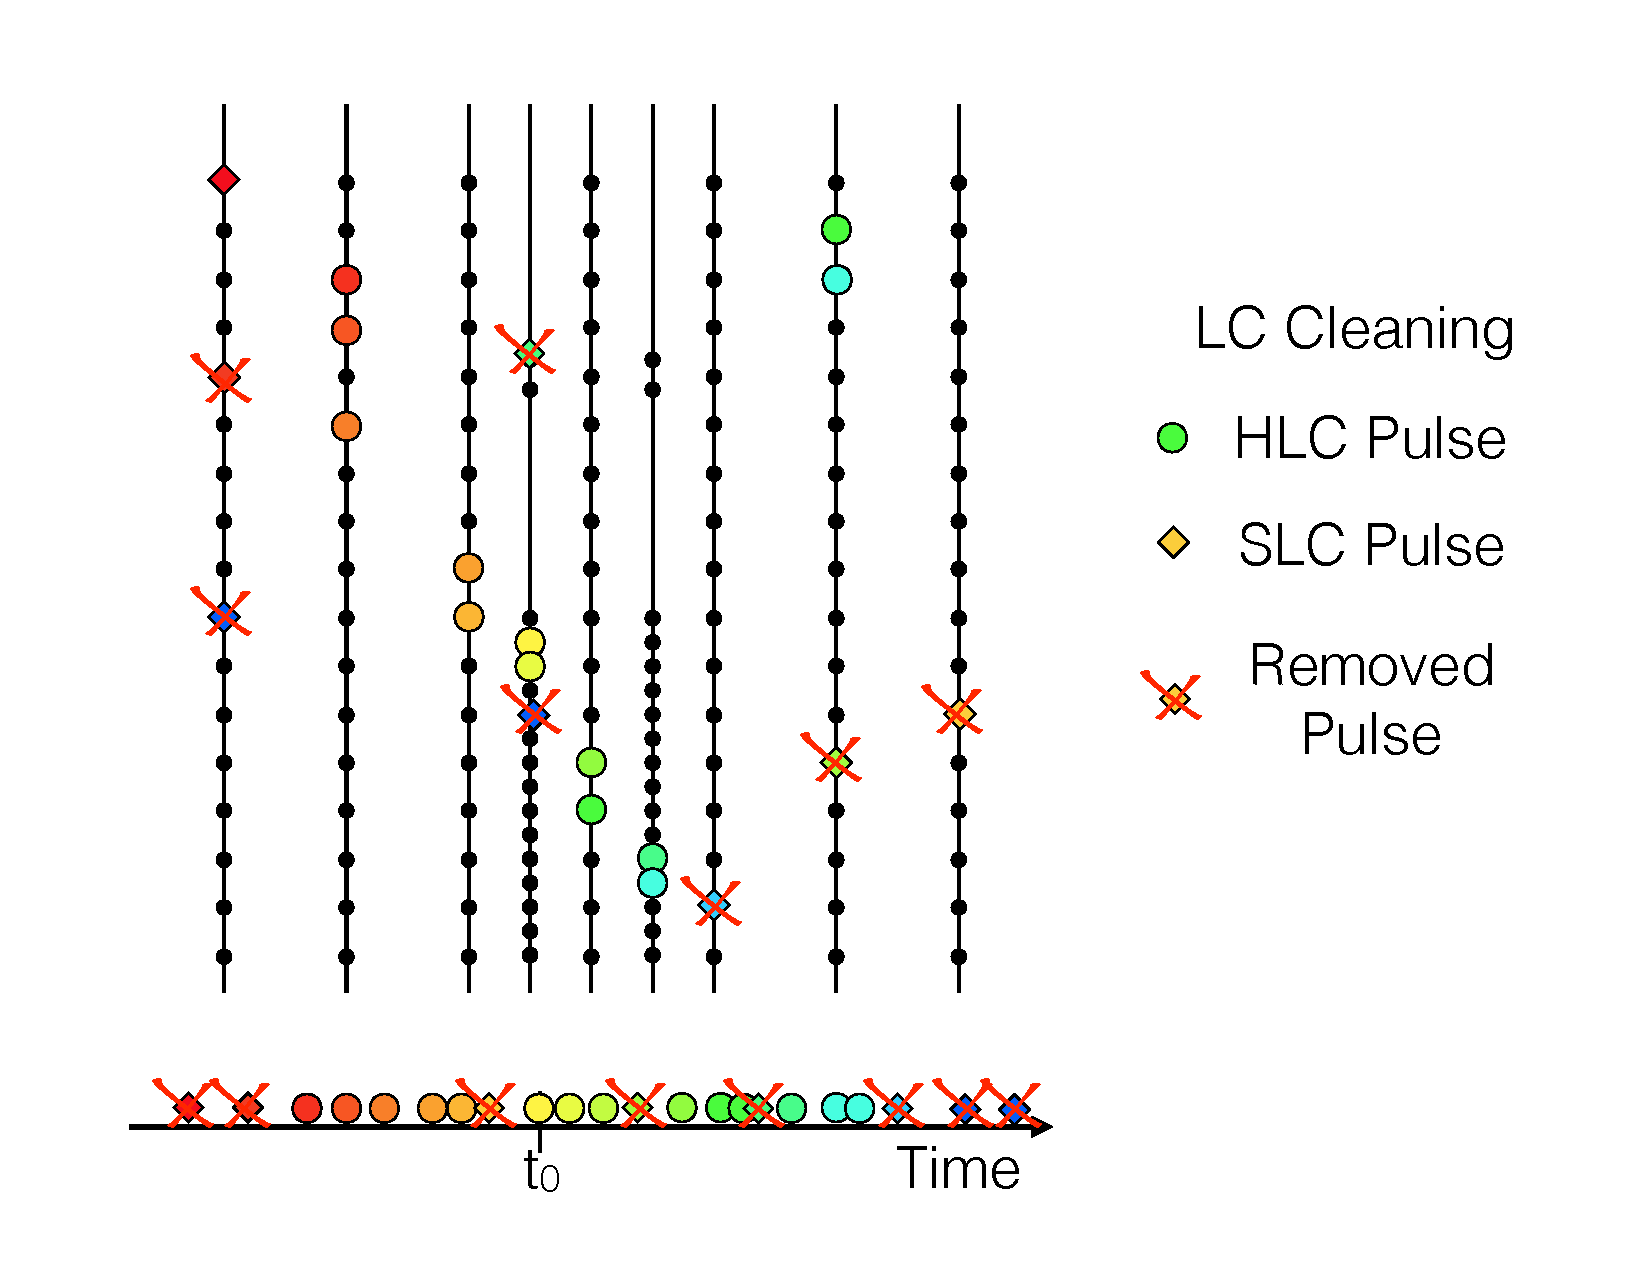
\includegraphics[width=0.3\textwidth]{LCCleaningDiagram.pdf}  &
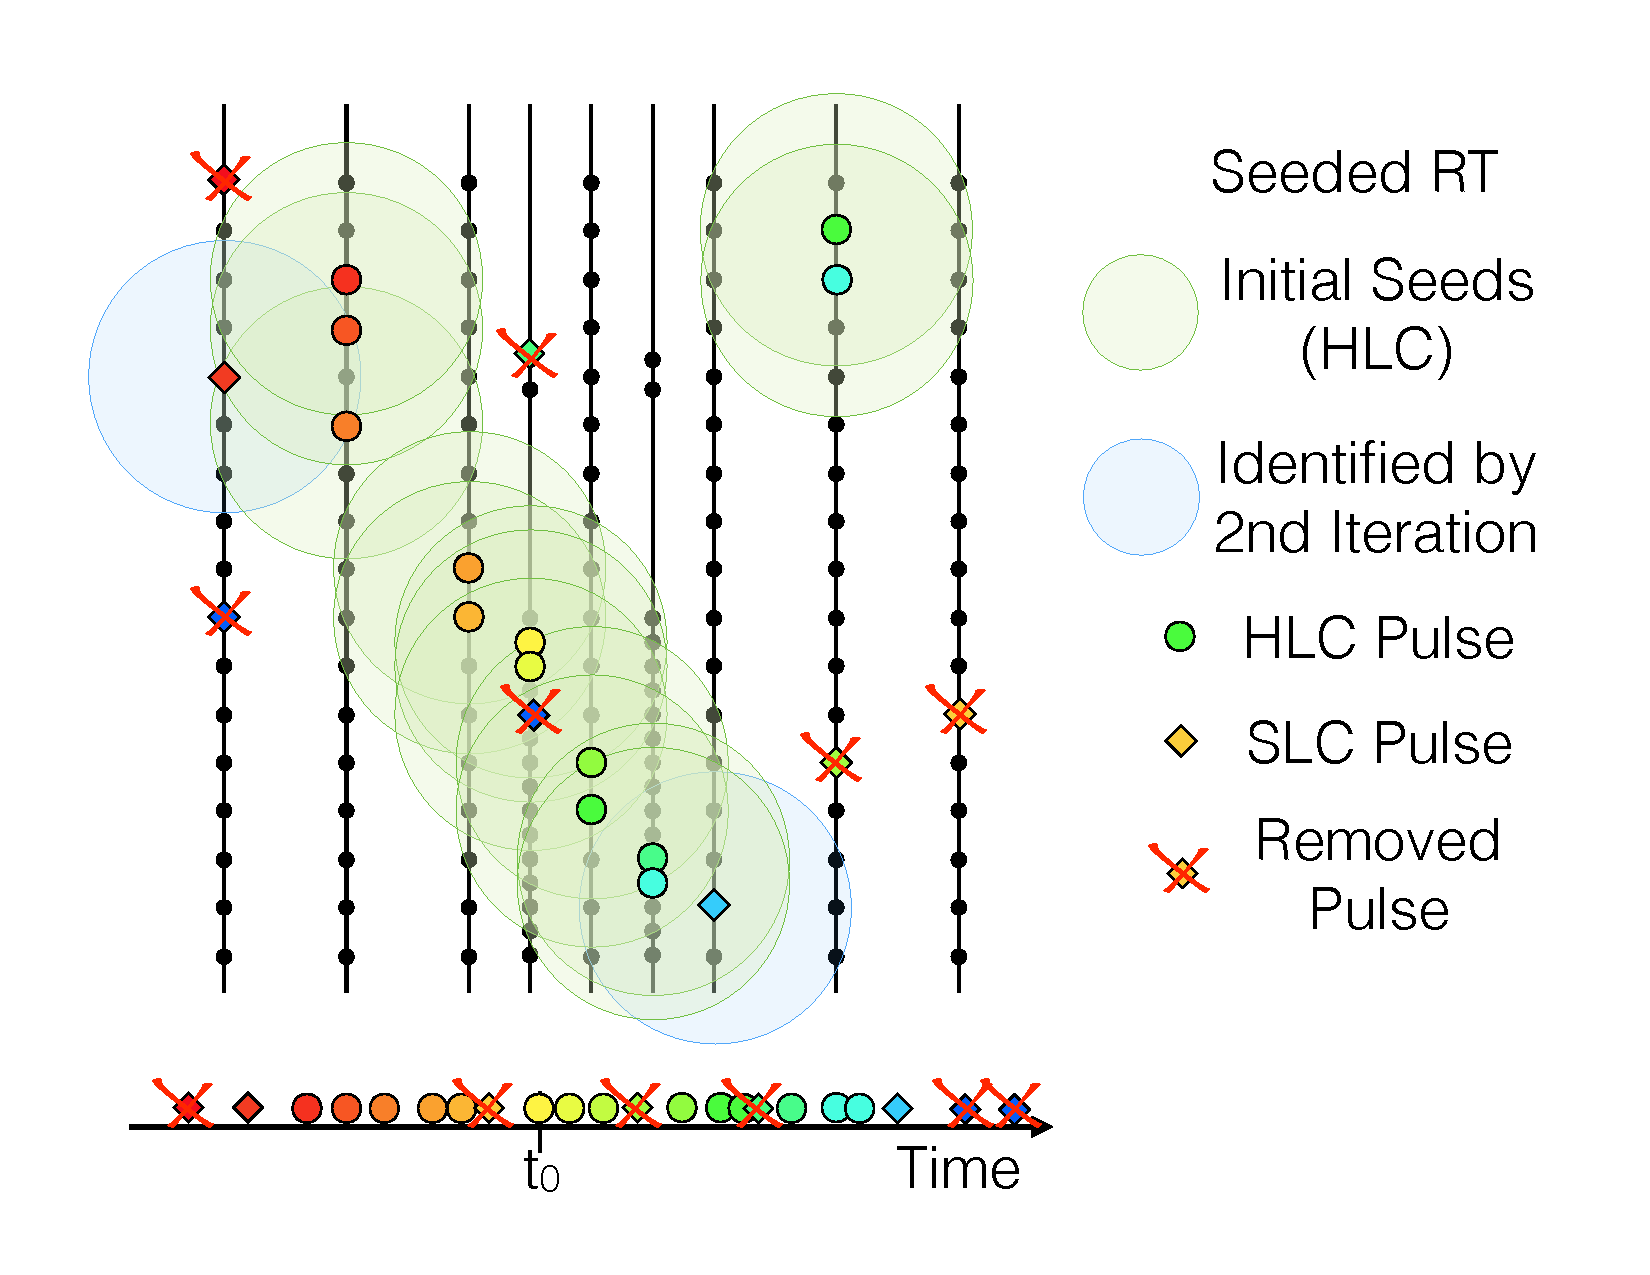
\includegraphics[width=0.3\textwidth]{SRTCleaningDiagram.pdf} & 
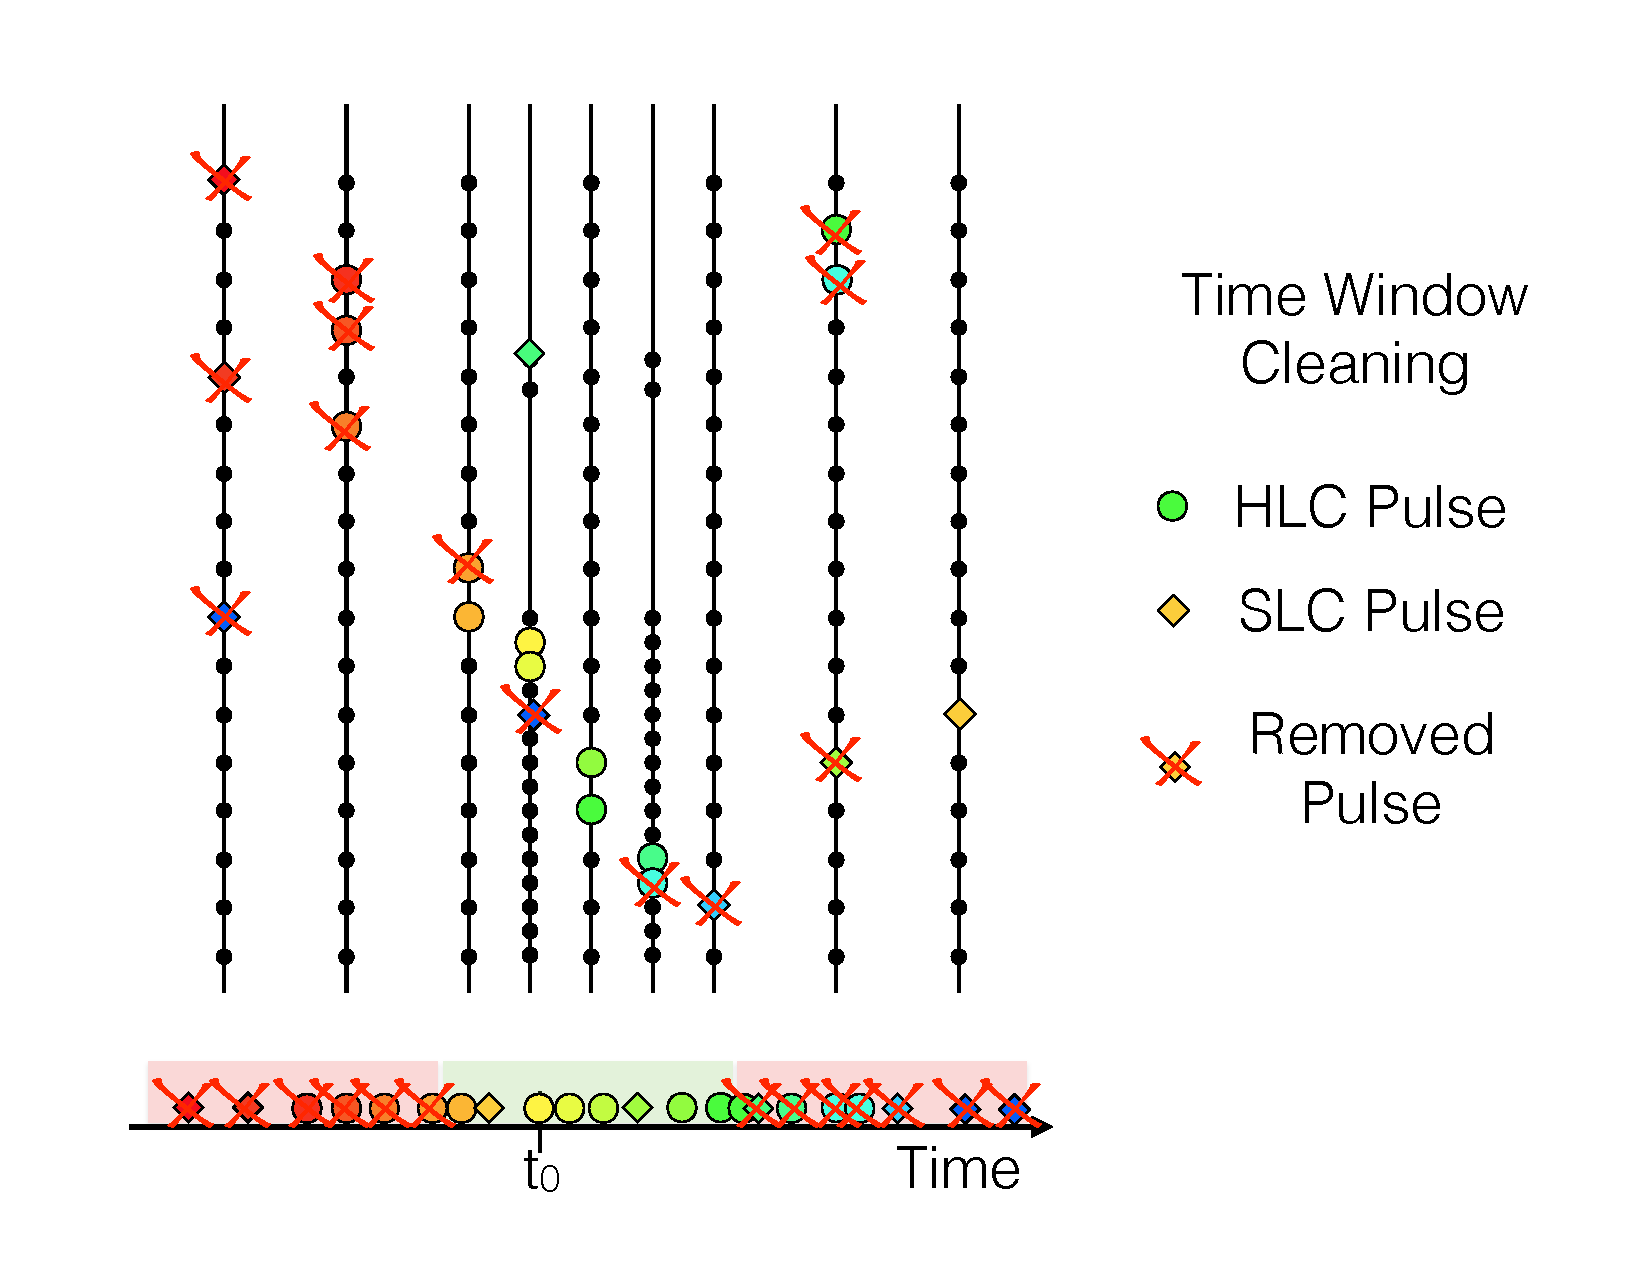
\includegraphics[width=0.3\textwidth]{TWCleaningDiagram.pdf}   	\\
\end{tabular}	
\caption{An illustration of the LC, SeededRT, and time window cleaning methods. (Left) All SLC pulses are removed while all HLC pulses are retained. (Middle) Pulses are removed based on time and distance from nearby HLC DOMs, allowing some SLC pulses to be accepted. (Right) Pulses are removed using the time relative to either the trigger (STW) or the maximum pulse density in time (DTW). }
\label{fig:hit_cleaning}
\end{figure}

\subsubsection{SeededRT Cleaning}
Instead of simply using HLC hits, additional processing may be used to identify potentially interesting SLC pulses as well.
The \emph{SeededRT} (\emph{SRT}) algorithm is one such algorithm, requiring a seed, radius, and time in order to search for additional information in the event as shown in Figure~\ref{fig:hit_cleaning}.
SeededRT begins with a subset of "interesting" pulses, often a selection of the HLC pulses, as a seed.
Once a seed is selected, a sphere is drawn around each seeded DOM. 
Any nearby DOMs within the sphere and time window are added to the output pulse series.
Once all seed DOMs have been checked, a new seed is created composed of the all current output pulse series.
The process is repeated until no further pulses are discovered.

The most effective set of parameters is dependent on the detector geometry, since a given radius sphere will contain more DOMs in the DeepCore fiducial than the same sphere outside of DeepCore.
Because of this, different settings are chosen for these two regions.
In the less dense IceCube detector, a typical value for the radius is 150 m and for the time window is 1000 ns. 
In DeepCore, these values are typically halved, with a raidus of 75 m and a time window of 500 ns.

The SeededRT algorithm is commonly used in IceCube, allowing for a pulse series with minimal noise contributions while finding most hits due to muon or neutrino interactions.

\subsubsection{Time Window Cleaning}
The most permissive pulse cleaning algorithm results in very little loss in pulses due to particle interactions, but allows nearly all noise pulses into the final hit series.
This \emph{Static Time Window} cleaning, often referred to using just the acronym \emph{STW} cleaning, looks for pulses near the time of the trigger.
For DeepCore processing, any pulses more than 4 microseconds before or more than 6 microseconds after the SMT3 time are removed.

There exists a second type of time window cleaning applied more rarely, but used in the GRECO selection.
The \emph{Dynamic Time Window} cleaning, hereafter \emph{DTW} cleaning, is a time window cleaning algorithm that uses the maximum pulse density in time to find the most likely interaction time of a muon or neutrino. 
The timing window is placed around this time instead of around the trigger.
DTW cleaning is generally chosen with a significantly tighter window, often consisting of only a few hundred nanoseconds compared to the multiple microseconds used in the STW cleaning.

Time window cleaning is typically used in combination with additional cleaning methods, resulting in little loss in useful signal due to the wide time window (in STW cleaning) or in a very pure set of hits likely to be due to unscattered light.

\label{sec:DeepCoreFilter}
\section{Level 1: The DeepCoreFilter}
Triggers are generally designed to be as accepting of the proposed physics signal as possible, regardless of the background rates.
Typically, limitations exist solely in the processing and storage capabilities in order to prevent the unintentional loss of valuable information.
After triggering, various filters may be applied with the sole purpose of removing the collected background.
For the purposes of this document, the only filter considered is the \emph{DeepCoreFilter}.

The DeepCoreFilter proceeds by splitting the pulses identified by the SeededRT cleaning into "veto" and "fiducial" pulses, with each DOM given a designation based on it's position in the detector as described in Section~\ref{sec:geometry} \cite{Description-DeepCore,Thesis-Vuvuzela}.
The average and standard deviation in time are first calculated for the fiducial pulses.
All hit DOMs with the first pulse occuring more than one standard deviation away from the mean time are removed from the fiducial pulse series in order to further limit the contributions from noise pulses.

With the updated fiducial pulse series, a center of gravity, or \emph{CoG}, of the remaining DOMs is calculated.

\begin{equation}
	\vec{x}_{CoG}=\frac{\sum_i^{DOMs} \vec{x}_i}{N_{hits}}
\end{equation}

The "corrected" average time of the fiducial pulses is then calculated by assuming that the pulse is due to light emission at the CoG, as would be the case for a point-like interaction of a cascade event.
\begin{equation}
	t_{CoG} = \frac{\sum_i^{DOMs} t_i^0 - \frac{\vec{x}_i - \vec{x}_{CoG}}{c_{ice}}}{N_{hits}}
\end{equation}

where $t_i^0$ denotes the time of the first observed pulse and $\vec{x}$ the position of each DOM.

All veto pulses are then compared to this CoG time and position by calculating an effective particle speed, $v$.

\begin{equation}
v = \frac{\left| \vec{x}_{COG} - \vec{x}_{hit} \right|}{t_{CoG} - t_{hit}}
\end{equation}

\begin{figure}
\centering
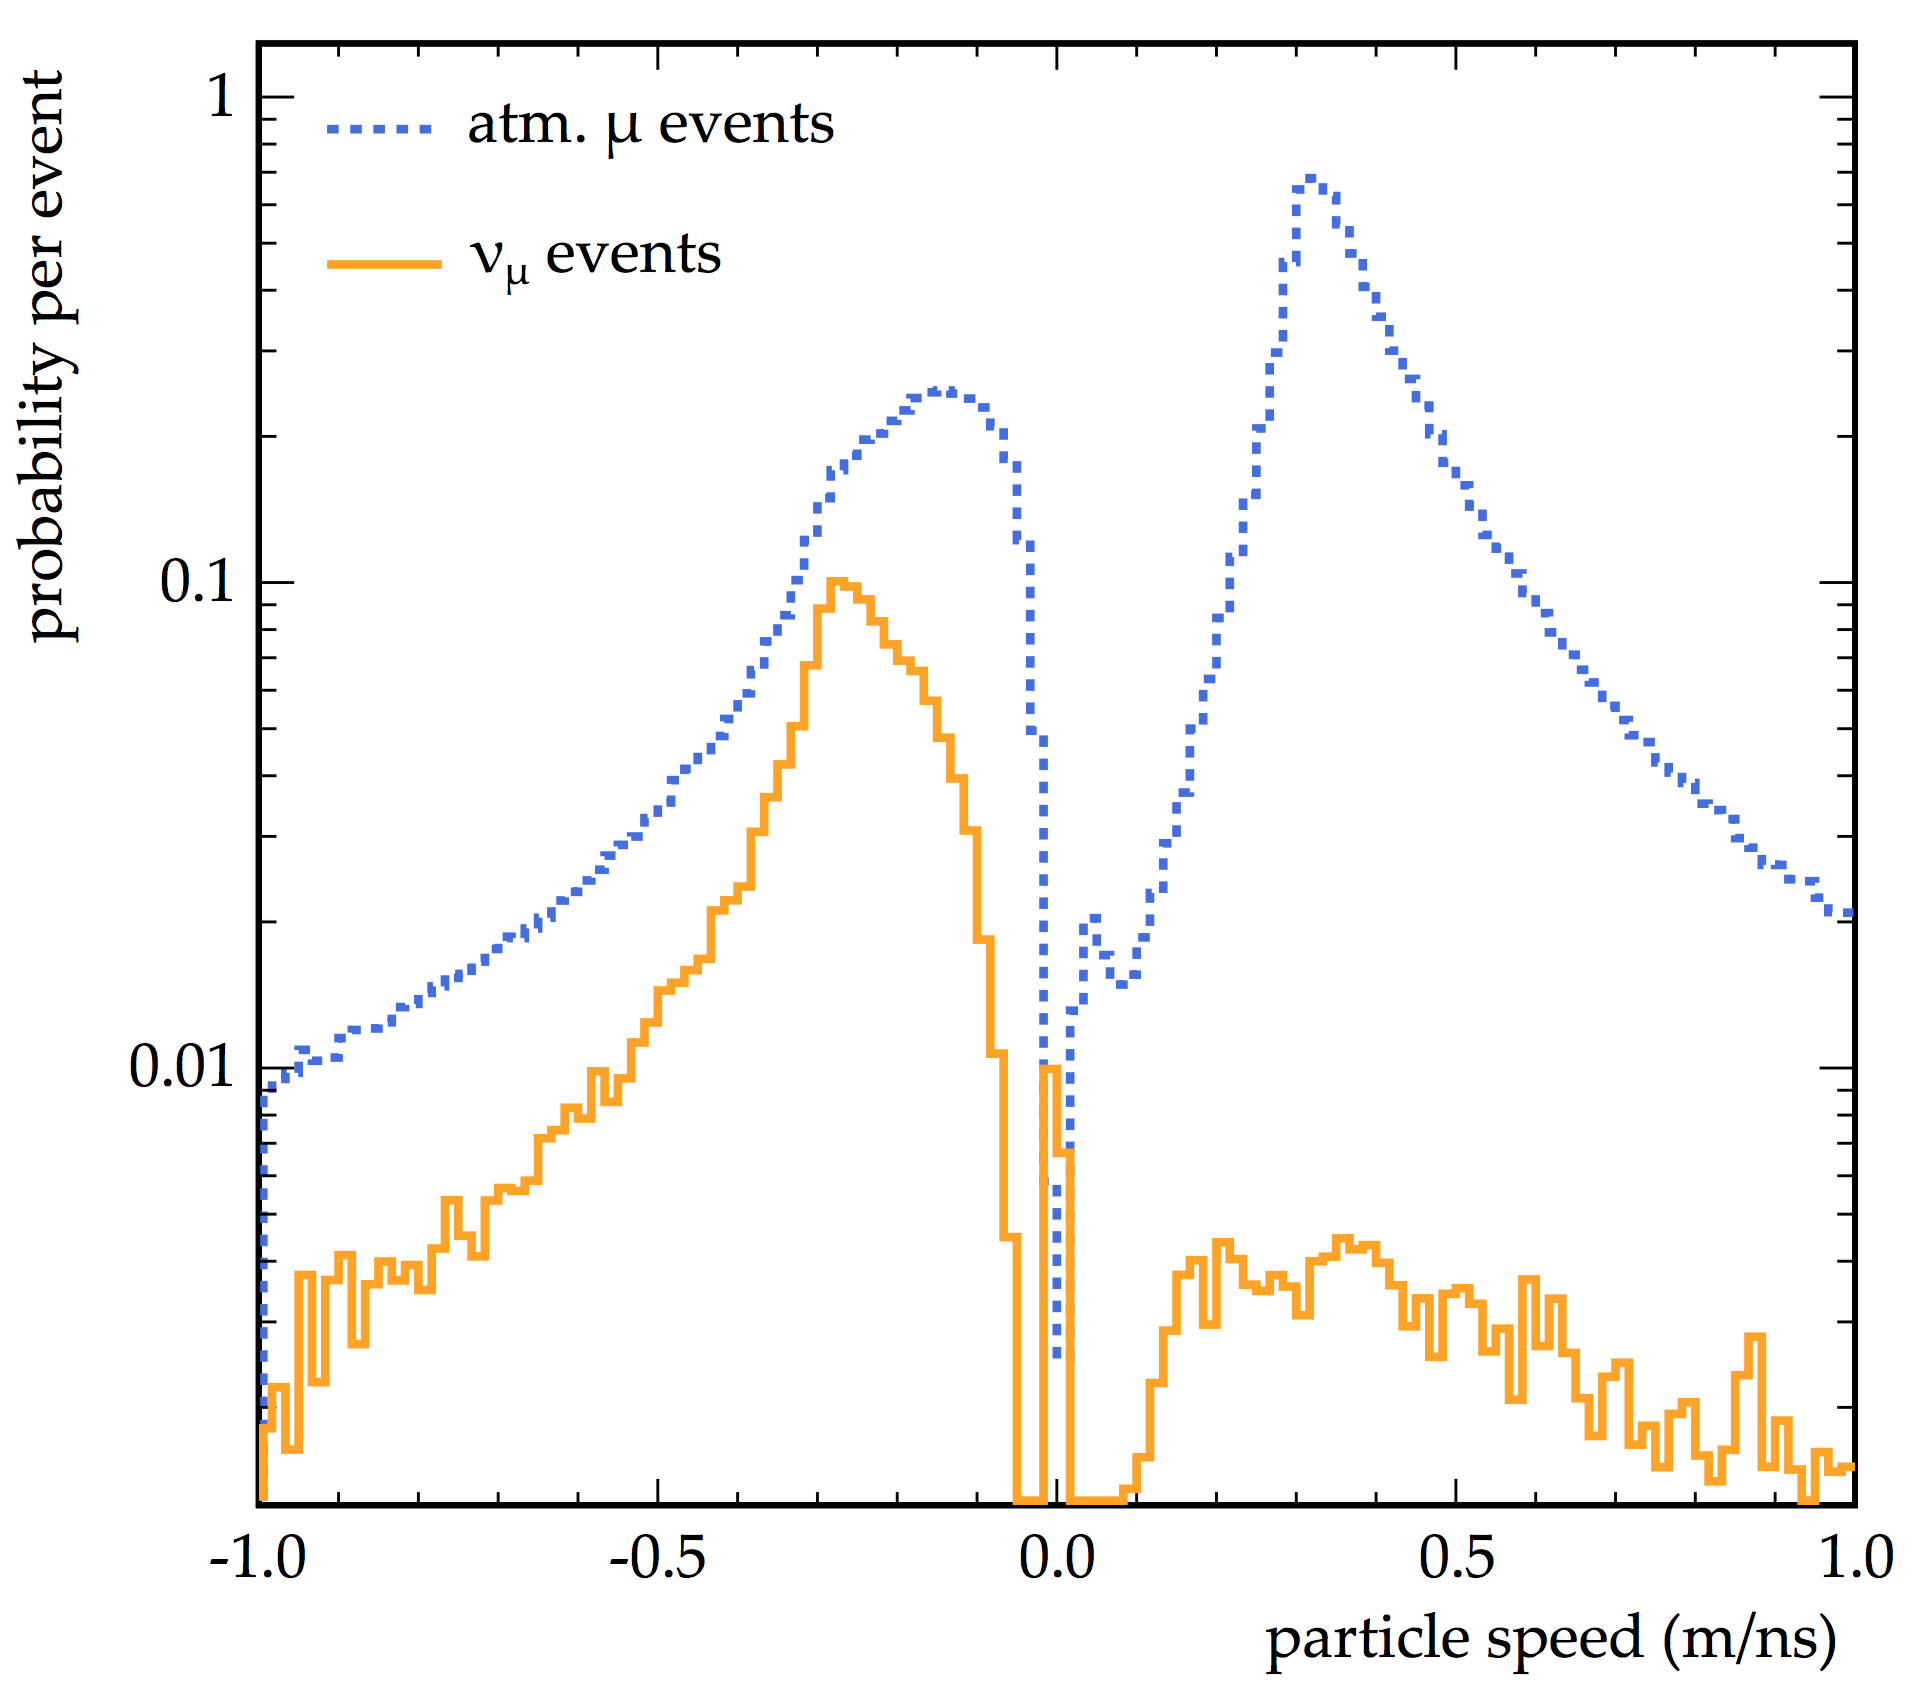
\includegraphics[width=0.7\textwidth]{deepcore_speeds.png}
\caption{The distribution of effective particle speeds used by the DeepCoreFilter to identify and reject muons. Because muons interact first outside of DeepCore, a large peak is visible at speeds around 0.3 m/ns, the speed of light. Figure from \cite{Description-DeepCore}}
\label{fig:deepcore_speeds}
\end{figure}

Muons passing through the detector will do so at the speed of light, 0.3 m/ns. 
Unscattered hits left behind in the detector show this peak clearly for muons.
Low energy neutrino events, on the other hand, typically begin in DeepCore, with hits outside of the fiducial region following hits inside. 
These neutrino events show a peak at negative speeds.

The DeepCoreFilter is the first step in a low energy analysis in IceCube and is used in many analyses \cite{Thesis-Vuvuzela,Thesis-Euler,IceCube-Oscillation2013,IceCube-Oscillation2015,IceCube-Oscillation2018}.
The algorithm reduces the atmospheric muon background from 280 Hz to approximately 17 Hz while retaining 99.4\% of neutrino events which begin in DeepCore \cite{Description-DeepCore}.

\graphicspath{{chapters/greco/images/level3/}}
\label{sec:level3}
\section{Low-En Level 3 Cuts}
After the DeepCoreFilter is used to remove events, variations of hit cleaning algorithms and reconstructions are used.
This processing stage, \emph{Level 2}, does not remove events from the selection and will not be discussed here.

Following the Level 2 processing, the \emph{Low energy Level 3} cuts are introduced.
These cuts are standardized and used in all DeepCore oscillation analyses.
The Level 3 processing stage introduces the structure of the remaining cut levels by using a set of \emph{accidental event cuts} and \emph{muon cuts}.

After the DeepCoreFilter, approximately half of the remaining rate consists of muons.
The remainder is due to accidental triggers due to random detector noise due to the low trigger threshold used in DeepCore.

\label{subsec:level3_noise}
\subsection{Accidental Rejection at L3}
Three cuts are introduced at Level3 in order to reduce the observed number of accidental triggers.
Events are required to have at least pulses and a total charge of at least 3 PE in a 250 ns DTW cleaned pulse series in the DeepCoreFiducial region.
This removes events which have reached Level 3 processing via random detector noise in the fiducial region.

In addition, the \emph{NoiseEngine} algorithm is used to identify accidental triggers \cite{Thesis-Vuvuzela}.
NoiseEngine uses the relative direction between each pair of hits to search for directionality of the event. 
Events with fewer than three hit pairs pointing in the same direction fail the algorithm and are rejected.
After the NoiseEngine algorithm, more than 96\% of accidental triggers are removed from the analysis.

\label{subsec:level3_muons}
\subsection{Muon Rejection at L3}
The removal of muons relies on some understanding of the characteristics of these events at Level 3.
Muons at this level are generally bright enough to be identified by hits in the outer part of the detector, known as the \emph{veto region}.
Because neutrino candidates of interest in this search are low energy, no light emission is expected in the veto region due to neutrinos.
This may be used to identify muons using cuts described here.

\subsubsection{First Hit Z Position}
Because the muon tracks are primarily steeply inclined, most will leave hits in the upper part of the detector.
Neutrinos of interest in the search for appearance will primarily emit light within the DeepCore fiducial volume, leading to little or no light emission in the top half of the detector. 
This difference between neutrino and muon emission in the upper part of the detector can be used to identify background muons
The position of the first hit in a STW+SRT cleaned pulse series consisting of DeepCore fiducial hits is used to look for muons using this principle.
Any event with a first hit above Z=-120 m is removed.

\subsubsection{NAbove200}
The total charge of recorded hits occuring in the top of the detector is also used in the analysis. 
This variable, known as \emph{NAbove200}, counts the amount of charge occuring before the SMT3 trigger above a depth of -200 meters.
If more than 12 DOMs are hit above Z=-200 m, then the event is removed.

\subsubsection{RTVeto}
The SeededRT algorithm is useful for removing accidental noise hits in the detector.
It may also be used to find clusters of hits due to muons in the outer part of the detector as well.
This technique, known as \emph{RTVeto}, uses the SeededRT algorithm to identify the largest cluster of pulses in the outer detector.
The number of hits in this cluster is used to identify atmospheric muon events.
The RTVeto algorithm uses a radius of 250 m and a time window of 1000 ns for both DeepCore and IceCube DOMs.

The cut is used in combination with the total amount of charge observed in the DeepCore fiducial region to define a few separate cut conditions.
For the purposes of this search, only the lowest energy version is relevent.
In this case, any event with a cluster of 4 or more hit DOMs in the outer detector is removed.

\subsubsection{C2QR6}
Atmospheric muon events at Level 3 tend to leave long tracks and take O(3 $\mu$s) to cross the detector.
Oscillation neutrino events prouce small light patterns small due to the low energies involved, with light being deposited quickly.
The difference in the light emission profile of the two event types may also be exploited to reject atmospheric muons background events.

To test the deposition time for light in each event, the \emph{charge ratio in 600 ns} (\emph{QR6}) is calculated as the ratio of charge observed in the first 600 ns and the total amount of observed charge.

\begin{equation}
QR6 = \frac{\sum_i^{t_i<600}} q_i}{\sum_i^{hits} q_i}
\end{equation}

Here the time is measured relative to the first observed hit in a STW+SRT pulse series.
Atmospheric muons will tend to deposit light over a longer timescale, resulting in a charge ratio near 0.
Neutrinos will deposit light quickly, with a charge ratio near 1.

The algorithm relies sensitively on the first observed hit.
The observation of noise hits before the particle interaction can lead to an erroneous definition of the time window.
In order to reduce this possibility, the first two hits may be ignored for the calculation. 
This form, the \emph{cleaned charge ratio in 600 ns} (\emph{C2QR6}) is used in the Level 3 processing to remove atmospheric muon events.

\subsection{Rates at Level 3}
\begin{table}[]
\centering
\begin{tabular}{@{}llll@{}}
\toprule
\multirow{2}{*}{Type} & \multicolumn{3}{l}{IceCube Processing} \\
                      & Any Filter   & DC Filter  & Low-en L3  \\ \midrule
CORSIKA               & 990598       & 9178       & 969.818    \\
MuonGun               & 60669        & 2982       & 442.493    \\
Accidentals           & 35855        & 8117       & 283.559    \\
$\nu_e$               & 1.842        & 1.721      & 1.262      \\
$\nu_{\mu}$           & 11.317       & 6.360      & 4.758      \\
$\nu_{\tau}$          & 0.293        & 0.270      & 0.206      \\ \midrule
MC Total*             & 1026466      & 17303      & 1260       \\
Data                  & 1154426      & 19092      & 1092       \\ \bottomrule
\end{tabular}
\caption{The event rates after the Level 3 cuts in GRECO. The total simulated rate is calculated using CORSIKA events and ignoring MuonGun. The data rate is estimated from a burn sample of 10 runs at Level 3. Rates are given in mHz.}
\label{tab:event_rates_L3}
\end{table}

The rates after the Level 3 cuts are applied is shown in Table~\ref{tab:event_rates_L3}. 
The atmospheric muons are reduced by about an order of magnitude.
The removal of accidental triggered events forms a large part of the reduction in rate at Level 3, with the rates decreased by more 96\%.


\graphicspath{{chapters/greco/images/level4/}}
\label{sec:level4}
\section{GRECO Level 4 Cuts}
The first GRECO-specific cut level is designated \emph{level 4}, or \emph{L4}, was first introduced in 2011 using very similar variables at the Level 3 cuts.
This is performed for historical reasons, as the DeepCore Level 3 and GRECO Level 4 were produced in parallel.

As in the DeepCore Level 3 processing, the GRECO Level 4 is divided into two types of cuts: those that remove accidental triggers due to detector noise and those that remove atmospheric muons. 
The cuts for atmospheric muons are then fed into a \emph{boosted decision tree} (\emph{BDT}), a multivariate algorithm designed to better separate signal from background \cite{TMVA}.
 
\subsection{Accidental Rejection at L4}
Similar to the cuts applied at Level 3, the GRECO Level 4 begins with a cut on the number of observed hits. 
In this case, static time window cleaning is applied with a range of $-3500 ns \leq t \leq 4000 ns$ for hits in the DeepCore fiducial volume.
A dynamic time window cleaning is then applied with a window of 200 ns.
Any events with fewer than three hits in this stricter pulse series is removed.

\subsection{Muon Rejection at L4}
Some cuts used to identify muons in the GRECO Level 4 are similar to those applied in the Level 3 processing. 
A stricter hit cleaning algorithm is used at this cut level to identify muons missed at Level 3.

\subsubsection{FirstHit Z}
\begin{figure}[h]
	\centering
		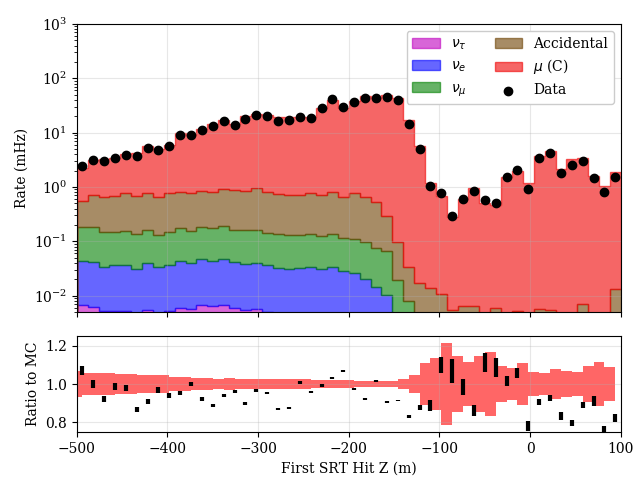
\includegraphics[width=2.5in]{FirstHitZ_log.png}
		\caption[The FirstHit Z position]{The Z position of the first hit in a cleaned hit series. Note the shape difference between the atmospheric muons in red and the various neutrino flavors, particularly above -200 meters.}
	\label{fig:firsthitz_log}
\end{figure}

The Z position of the first hit DOM in the event is included for the GRECO Level4. 
The cut continues to show separation between neutrino events and atmospheric muons with the new hit cleaning.

\subsubsection{NAbove200}
\begin{figure}[h]
	\centering
		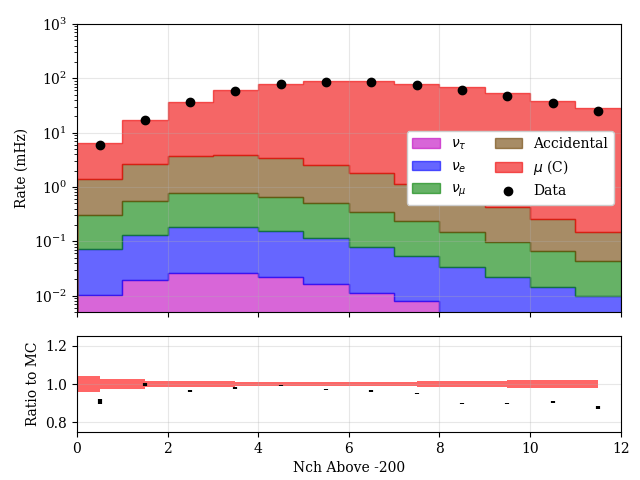
\includegraphics[width=2.5in]{NAbove200_log.png}
		\caption[Number of Hits Above Z=-200]{The number of hits above Z=-200 meters}
	\label{fig:nabove200_log}
\end{figure}

Similarly, the number of hit DOMs identified above Z=-200 m is again used with a new hit series.
Once again, some separating power remains.

\subsubsection{QR6/C2QR6}
\begin{figure}{h}%
	\centering
		\subfloat[QR6]{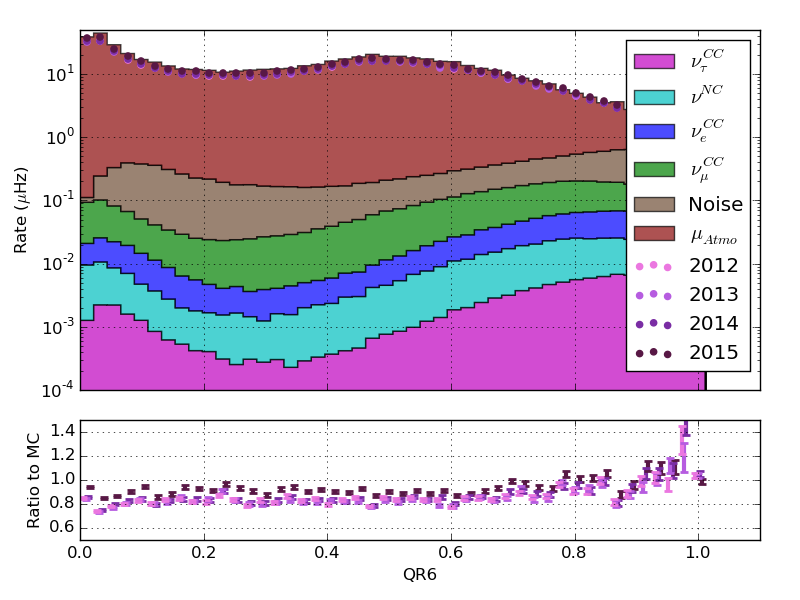
\includegraphics[width=2.3in]{QR6_log.png}}%
		\subfloat[C2QR6]{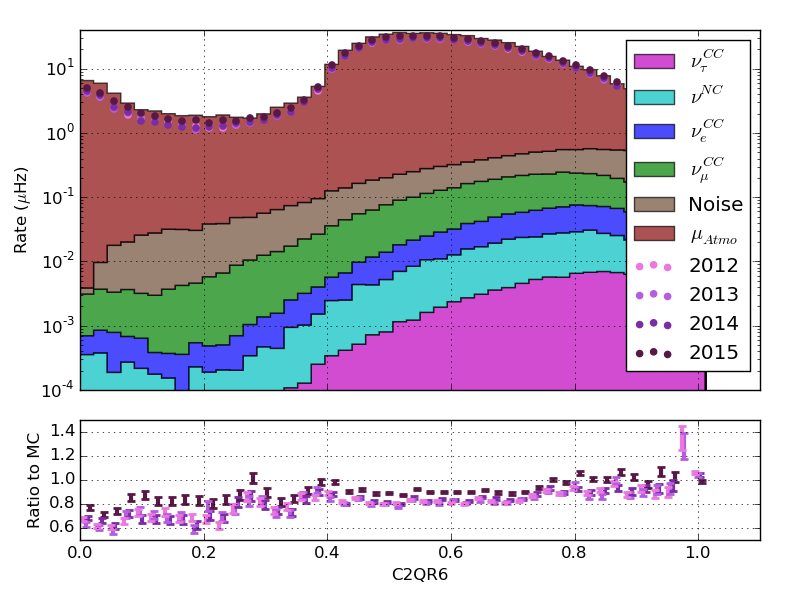
\includegraphics[width=2.3in]{C2QR6_log.png}}%
	\caption[QR6 and C2QR6]{The charge ratio variables used in the L4 cuts.}%
	\label{fig:QR6_and_C2QR6}%
\end{figure}

Both the QR6 and C2QR6 are used in the GRECO Level 4 processing. 
The two show some degeneracy, although the BDT training suffers if only one is available.
Note that there exists some significant disagreement between data and simulation at low values of C2QR6.
This region does not contain much signal and will be removed by the BDT.

\subsubsection{Tensor of Inertia}
\begin{figure}[h]
	\centering
		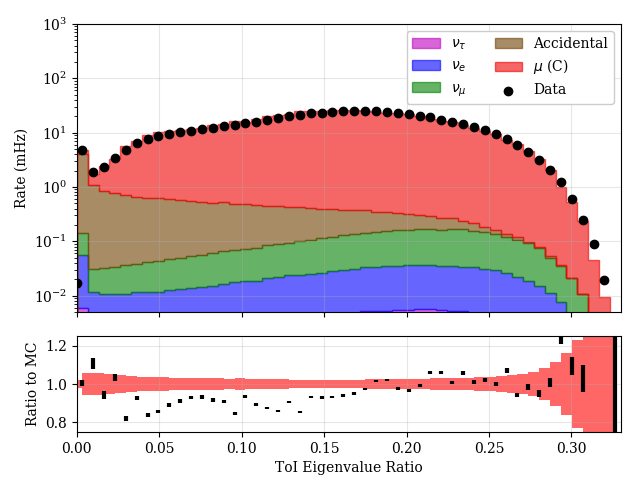
\includegraphics[width=2.5in]{ToIEval_log.png}
		\caption[Tensor-of-Inertia Eigenvalue Ratio]{The eigenvalue ratio from a ToI calculation. Larger values indicate more apparent elongation in the event.}
	\label{fig:toi_log}
\end{figure}

At this early level, the shape difference in the observed hit pattern will be relatively clear.
Many neutrinos with energies in the range of 1-100 GeV will appear to be rather small and compact in DeepCore forming a cascade-like event.
Muons will have a longer visible track.
These differences may be interpreted via use of the \emph{Tensor of Inertia eigenvalue ratio} (more briefly, \emph{ToI}).
This variable is defined in analogously to the tensor of inertia from mechanics, with the measured charge taking the place of the mass.

\begin{equation}
\begin{tabular}{c}
	I_{X} = \sum_{i=0}^{nhits}(y_i^2 + z_i^2)q_i	\\ \\
	I_{Y} = \sum_{i=0}^{nhits}(x_i^2 + z_i^2)q_i \\ \\
	I_{Z} = \sum_{i=0}^{nhits}(x_i^2 + y_i^2)q_i \\
\end{tabular}
\end{equation}

These three moments yield information about the shape of the event.
The eigenvalue ratio is defined as 

\begin{equation}
	e = \frac{\mathtt{max}(I_j)}{I_{x}+I_{y}+I_{z}}
\end{equation}

Events which are very track-like, and therefore muon-like, have eigenvalue ratios near 0 while more cascade-like events have eigenvalue ratios close to $\frac{1}{3}$.


\subsubsection{Linefit Speed}
\begin{figure}[h]
	\centering
		\includegraphics[width=2.5in]{iLineFit_Log.png}
		\caption[The improvedLineFit Speed]{The apparent speed, in units of meters per nanosecond, corresponding to the hits in the event. Faster speeds are associated with particle travel instead of light travel.}
	\label{fig:ilinefit_log}
\end{figure}

The \emph{line fit} is an first-guess reconstruction used in IceCube.
The algorithm assumes that the hit pattern in an event may be modeled as a plane wave passing through the detector at speed $\vec{v_{LF}}$.
The speed of the plane wave may be solved analytically \cite{LineFit}.

\begin{equation}
\vec{v_{LF}} = \frac{\left<t_i \cdot \vec{x_i} \right> - \left<\vec{x_i}\right>\left<t_i\right>}{\left<t^2\right> - \left<t_i\right>^2}
\end{equation}

where $\left<t_i\right>$ denotes the average hit time.
Cascade-like events have hits moving without a preferred direction while the atmospheric muons have a single preferred direction.
Using the line fit speed, the neutrino sample is expected to have a speed closer to 0 while the atmospheric muons show a speed closer to the speed of light, 0.3 m/ns.

\subsubsection{The L4 BDT}
\begin{figure}[h]
	\centering
		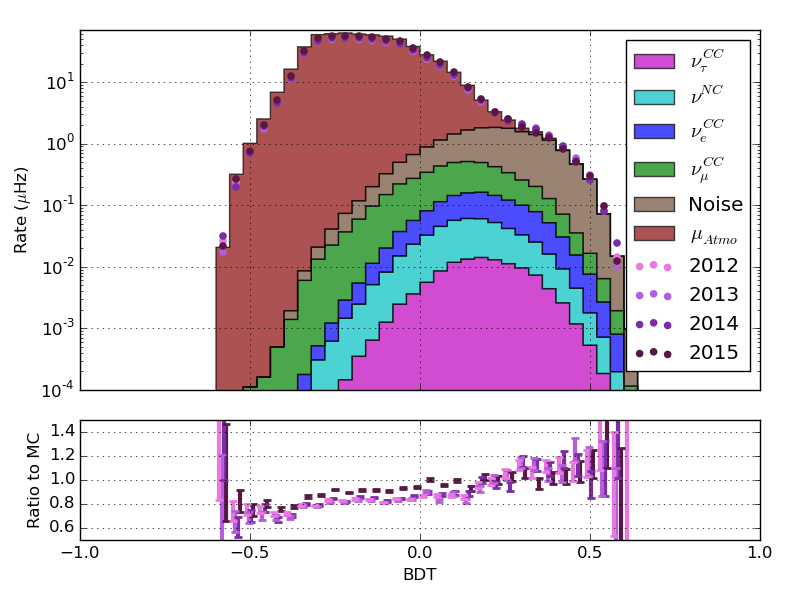
\includegraphics[width=0.9\linewidth]{BDT_log.png}
		\caption[The L4 BDT Score]{The distribution of the boosted decision tree used at L4. A cut is applied at 0.04 to remove a significant fraction of atmospheric muon background events. Note the ratio, which shows disagreement in the very muon-like region. The region of disagreement is removed by the cut.}
	\label{fig:L4_bdt_log}
\end{figure}

A Boosted Decision Tree (\emph{BDT}) is trained at L4 to further reduce the atmospheric muon background by a factor of 10x. 
The variables described above were provided to a BDT training using the CORSIKA as the background training sample and GENIE simulation as the signal sample. 
The BDT uses a series of \emph{trees}, collections of multidimensional cuts, to classify events as either signal-like or background-like \cite{TMVA}.
After \emph{boosting}, a process by which event weights are adjusted based on the success or failure of previous classification attempts.
The BDT returns a \emph{score} ranging from -1 (background-like) to +1 (signal-like) which may be used as a cut variable in an analysis.

The score returned by the GRECO Level 4 BDT is shown in Figure\ref{fig:L4_bdt_log}.
The distribution ranges from -0.6 to +0.6, indicating that no signal or background events are perfectly identifiable.
Separation is observed between the atmospheric muon events, which peak around a score of -0.25, and signal, peaking at +0.15.

Comparisons to MC show mild disagreement, particularly in the most muon-like regions that get cut away. 
Its not obvious what causes the disagreement, although it is possible that the assumed cosmic ray flux model is simply an inaccurate model of some part of the spectrum that contributes. 
Alternatively, this may be an artifact of undiscovered mismodeling of the atmospheric muon events.
Differences in the high energy muon events would likely have clear tracks visible in the detector, contributing to the region around -0.5.
No investigation of the disagreement has been performed, as these events are removed from the GRECO selection.

A shoulder attributable to the accidental triggers is visible at high values of the BDT score, peaking around 0.25, indicating that these events appear more signal-like than the nuetrino samples.
While initially puzzling, investigation of the training of the BDT showed that the original training sample did not include these events.
Instead, only CORSIKA and GENIE events were used to train the BDT.
Because the training lacked any accidental triggers as a reference, the BDT picked the most obvious feature of the GENIE sets: that the signal events were primarily low energy with lower light deposition than the background. 
These are also key features of the noise triggers. 

The GRECO Level 4 places a cut at 0.04 in the BDT score, removing a large fraction of the background sample.
A large fraction of the neutrino sample is also removed in order to reduce the muon rates by a factor of 20x.

\subsection{Rates at Level 4}
\begin{table}[]
\centering
\begin{tabular}{@{}lllll@{}}
\toprule
Type         & \multicolumn{3}{l}{IceCube Processing} & GRECO  \\
             & Any Filter   & DC Filter  & Low-en L3  & L4     \\ \midrule
CORSIKA      & 990598       & 9178       & 969.818    & 50.511 \\
MuonGun      & 60669        & 2982       & 442.493    & 33.562 \\
Accidentals  & 35855        & 8117       & 283.559    & 11.963 \\
$\nu_e$      & 1.842        & 1.721      & 1.262      & 0.783  \\
$\nu_{\mu}$  & 11.317       & 6.360      & 4.758      & 2.503  \\
$\nu_{\tau}$ & 0.293        & 0.270      & 0.206      & 0.134  \\ \midrule
MC Total*    & 1026466      & 17303      & 1260       & 65.893 \\
Data         & 1154426      & 19092      & 1092       & 68.592 \\ \bottomrule
\end{tabular}
\caption{The event rates after the Level 4 cuts in GRECO.  The total simulated rate is calculated using CORSIKA events and ignoring MuonGun. The data rate is estimated from a burn sample of 30 runs at Level 4. Rates are given in mHz.}
\label{tab:event_rates_L4}
\end{table}

The rates of the selection after the Level 4 cuts are applied is shown in Table~\ref{tab:event_rates_L4}.
After the GRECO Level 4 BDT, the number of atmospheric muons is reduced to 50 Hz, a mere 25x the muon neutrino rate.
The number of accidental triggers is also reduced in the analysis due to the dedicated cuts applied at this level.
The number of accidental triggers is still larger than the number of neutrinos expected, however, indicating that further cuts are necessary.












\graphicspath{{chapters/greco/images/level5/}}
\label{sec:level5}
\section{Level 5 Cuts}
The next stage of cuts, know as the \emph{GRECO Level 5}, or more simply, \emph{L5}, also uses a BDT.

\subsection{Accidental Rejection at L5}
Unlike the previous stages, however, there is no explicit cut introduced at L5 to remove accidental triggers.
Instead, an implicit requirement on the number of hit DOMs arises due to the the reconstruction used at Level 5.
The STW+SRT pulse series containing DeepCore fiducial pulses is used to fit a total of 6 free parameters.
The parameters are degenerate if fewer than five hits are used.
In this case, the reconstruction fails to converge and the event is removed.
Because of this degeneracy, the GRECO Level 5 implicitly requires at laest 6 hit DOMs in this hit series.

\subsection{Muon Rejection at L5}

\subsubsection{Time to 75\% Charge}
\begin{figure}[h]
	\centering
		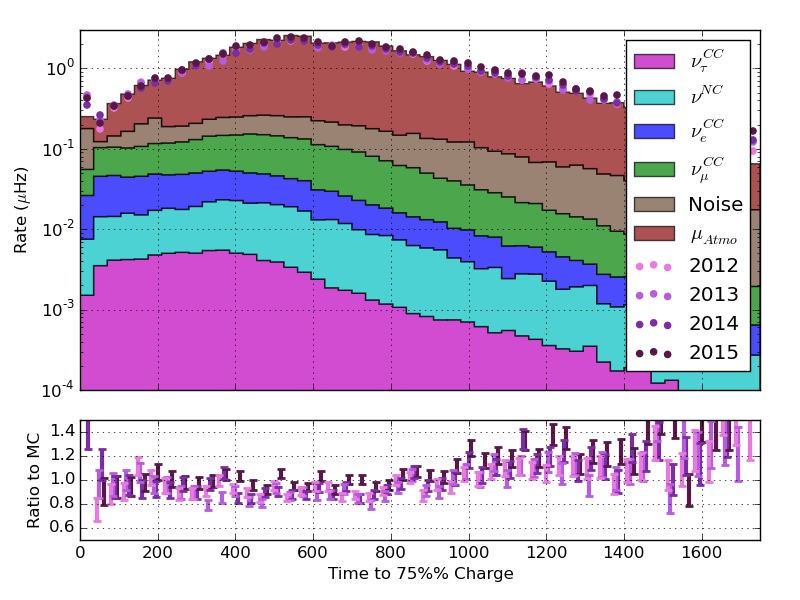
\includegraphics[width=2.5in]{Time_to_75_Charge_log.png}
		\caption[Time to 75\% Charge]{The time to accumulate 75\% of the total charge of the event.}
	\label{fig:time_to_75}
\end{figure}

The first variable used to create the L5 BDT is the amount of time requried to deposit 75\% of the total charge, the \emph{$t_{75}$}. 
Similar to the QR6 and C2QR6 variables, the $t_{75}$ is a variable designed to look at the hit distribution in time.
However, the variable is now produced in the reverse manner: where the QR6 variable refers to the amount of a charge in a given window, the $t_{75}$ instead attempts to find the amount of time for a given charge level.
The providing an on the total event length and timing distribution.

The neutrino events deposit energy quickly due to the low energies of the sample of interest in this thesis.
The muon events take longer to reach 75\% of the total charge due to the long travel time of the events through the detector.

\subsubsection{Veto Identified Causal Hits}

\begin{figure}[h]
\centering
  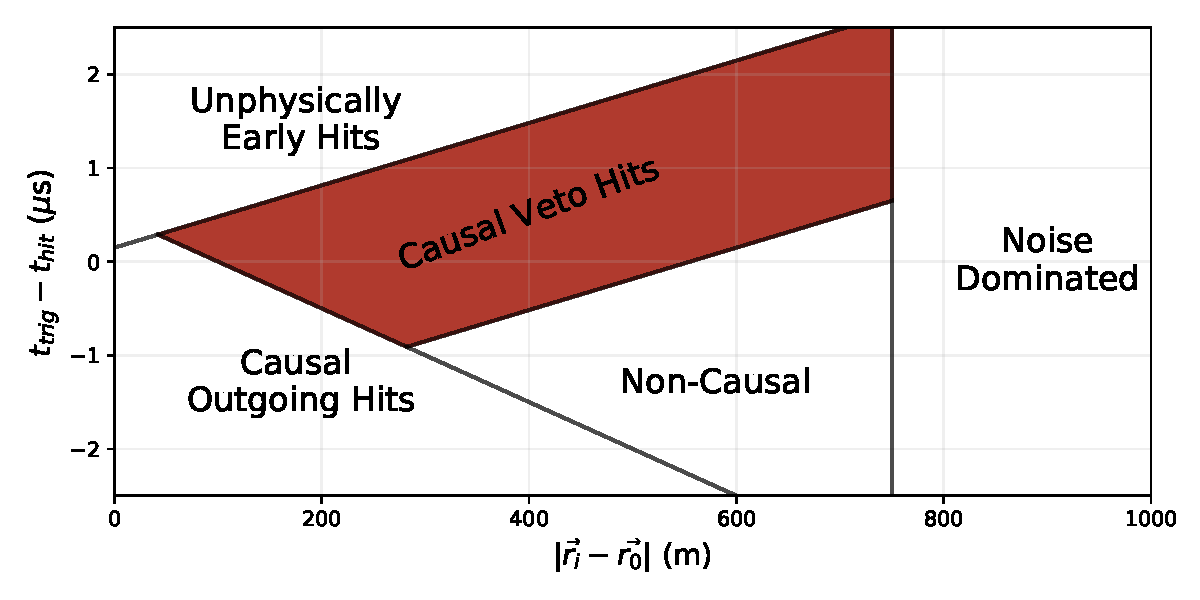
\includegraphics[width=0.45\linewidth]{vich_diagram.pdf} \\
\caption{A schematic diagram showing the regions of the VICH algorithm. VICH returns the number of hit DOMs in the shaded region, corresponding to the pulses that are both causally connected with the trigger and entering DeepCore. }
\label{fig:vich_diagram}
\end{figure}

\begin{figure}[h]
	\centering
		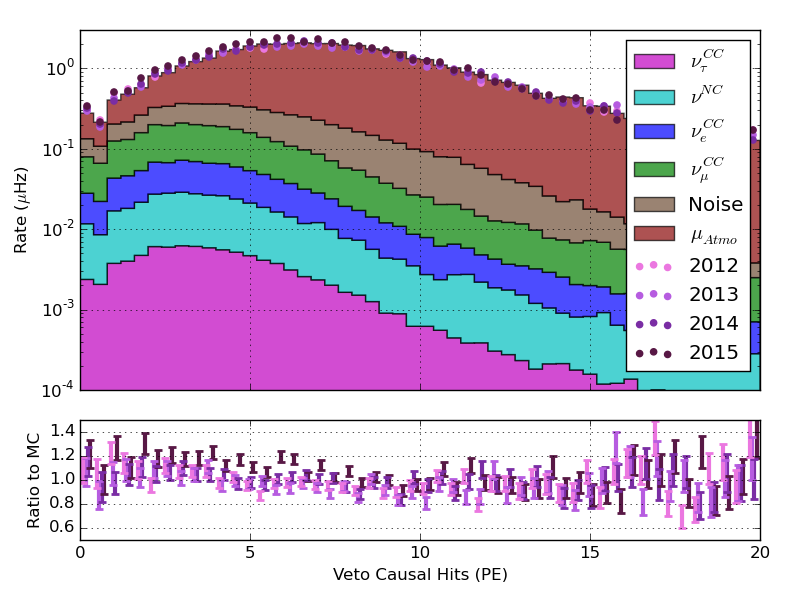
\includegraphics[width=2.5in]{Veto_Causal_Hits_(PE)_log.png}
		\caption[Veto Identified Causal Hits]{The amount of causally-connected charge discovered in the veto region.}
	\label{fig:vich}
\end{figure}

The \emph{Veto Identified Causal Hits} (\emph{VICH}) algorithm is also used in the GRECO Level 5.
This algorithm uses an uncleaned hit series to search for hits that are causally connected to the trigger \cite{Thesis-Euler}.
The first DOM to contribute to the DeepCore trigger is used to define the trigger time and position.

Five regions are defined based on various criteria shown in Figure~\ref{fig:vich_diagram}.
Hits which are not causally connected to the trigger are ignored. 
Hits which occur too far away from DeepCore are also ignored to reduce the effect of detector noise.
A causal region which is consistent with light travel outgoing from the trigger position is also ignored.

The VICH algorithm returns the number of hits in the remaining "causal veto region".

\subsubsection{First Hit $\rho$}
\begin{figure}[h]
	\centering
		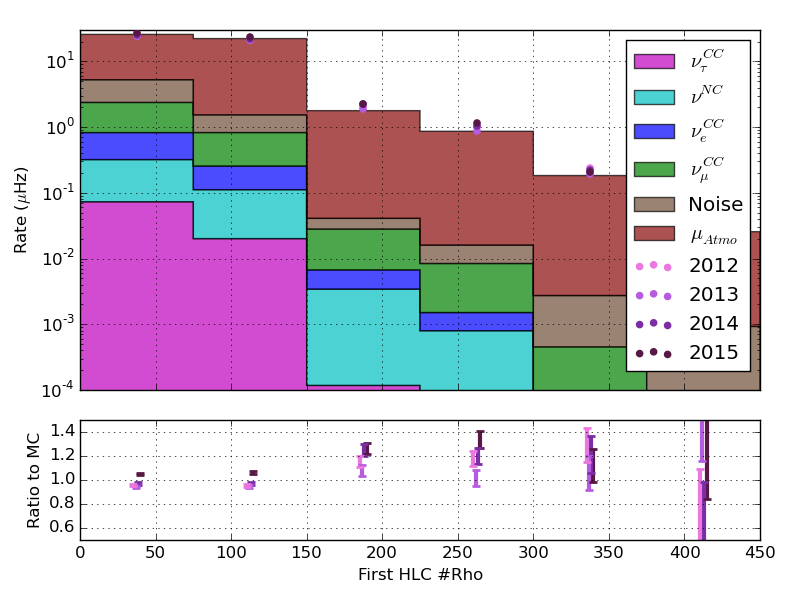
\includegraphics[width=2.5in]{First_HLC_Rho_log.png}
		\caption[First Hit $\rho$ Position]{The radial position of the earliest hit of a cleaned hit series. The radial position is measured relative to string 36, the center of DeepCore.}
	\label{fig:firsthit_rho}
\end{figure}

The Z position of the first hit was used in the GRECO Level 4 cuts in order to indentify atmospheric muons coming from above DeepCore.
The X and Y position may also be used to identify muons.
These are combined to define a \emph{radial distance} (\emph{$\rho_{36}$}) from the center of DeepCore, here defined to be the position of string 36 at $(x,y)=(46.3, -34.9)$.

\begin{equation}
\rho_{36} = \sqrt{\left(x-x_0\right)^2 + \left(y-y_0\right)^2}
\end{equation}

The radial distance is a general parameter and can be used with any event vertex. 
For the GRECO Level 5, the first hit in the STW+SRT pulse series is used.
Atmospheric muons entering DeepCore are more likely to be found at larger values of $rho_{36}$ while neutrinos are more likely to be found within the DeepCore fiducial volume, which stops at $rho_{36}=125$.

\subsubsection{Quartiles CoG}
\begin{figure}[h]
	\centering
		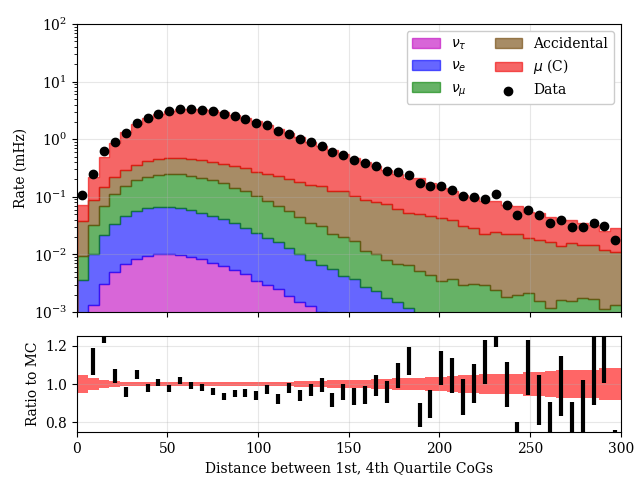
\includegraphics[width=2.5in]{Q1-Q4_Distance_log.png}
		\caption[Quartile Distance]{The distance between the centers of gravity of the first and last quartile in time.}
	\label{fig:quartile_distance}
\end{figure}

The distance traveled by muons may be exploited as well.
In particular, a track-like event is expected to travel over a longer distance than a cascade-like event of a similar energy.
In GRECO Level 5, the distance between the CoGs of the first and last quartiles in time are used to characterize the distance traveled by the interaction.
For atmospheric muon events, this distance is expected to be larger than for low energy neutrino events.

\subsubsection{Z-Travel}
\begin{figure}[h]
	\centering
		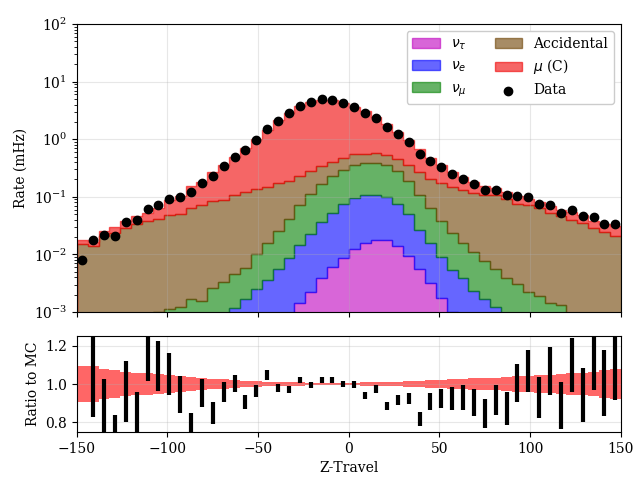
\includegraphics[width=2.5in]{Z-Travel_log.png}
		\caption[Quartile Z-Travel]{The distance traveled in Z between the first and last quartile of hits in time.}
	\label{fig:quartile_ztravel}
\end{figure}

The total distance traveled in the detector is only one useful measure that may be calculated using the quantiles in time.
Another useful metric is the distance traveled only in the Z coordinate. 
The value, known as the \emph{z-travel}, is a measure of the direction of the particle

\begin{equation}
\Delta Z = Z_{Last} - Z_{First} 
\end{equation}

The z-travel is typically used to identify atmospheric muons.
Atmospheric muons traveling through the detector from above will have a negative z-travel distance and neutrinos may be positive or negative, but is likely to be small due to the small size of neutrino events.

The accidental triggers also are also well-separated from the simulated neutrinos.
These events do not have a preferred direction and appear at all values of the z-travel and appear at all values.
The accidental events dominate at the tails of the distribution.

\subsubsection{SPE Zenith}
\begin{figure}[h]
	\centering
		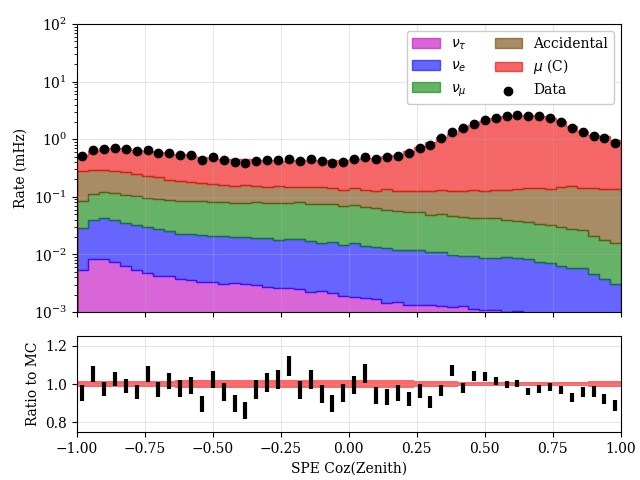
\includegraphics[width=2.5in]{SPE11_Cos(Zenith)_log.png}
		\caption[SPE Reconstruction Zenith Angles]{The zenith angle distribution of events from an 11-iteration SPE fit. The fit assumes an infinite track hypothesis and uses only hit DOMs.}
	\label{fig:spe11_zenith}
\end{figure}

More advanced reconstructions are viable at this level, providing new potential for the identification of atmospheric muons from neutrino candidates.
These reconstructions must account for the effects of scattering in order to produce meaningful results.

The time required for a Cherenkov photon to reach a DOM from a point-like emission is 

\begin{equation}
t_{point} = t_{emission} + \frac{n}{c} \left|\vec{r}\right| 
\end{equation}

where $\left|\vec{r}\right|$ is the distance between the emission point and the DOM.
The corresponding time from a muon track is 

\begin{equation}
t_{track} = t_{emission} + \frac{\vec{r} \cdot \hat{n} + \rho \tan \theta_C}{c}
\end{equation}

where $\hat{n}$ is a unit vector pointing in the direction of the muon track, $\theta_C$ is the Cherenkov angle, and $\rho = \left|\vec{r} - \left(\vec{r} \cdot \hat{n}\right) \hat{n}\right|$ is the impact parameter of the track with respect to the DOM \cite{Thesis-Jakob}.
In the absence of scattering, all photons would arrive at the DOM according to these times.
The addition of scattering delays photons, as they travel a greater distance before reaching the DOM.
These delayed photons give a \emph{time residual} distribution.

There is no analytic form for the timing which includes the effects of scattering, although approximations exist.
One such approximation, the Pandel function \cite{Thesis-Pandel}, may be used to estimate the time residual distributions as a function of source-reciever distances \cite{Pandel_SPE}.

The Pandel functions may be used to construct a likelihood of the form

\begin{equation}
L\left(x_{vertex}, t_{vertex}, \hat{n}\right) = 
 \prod_{i}^{pulses} \frac{dP_{Pandel}\left(t_i-t_{point} | x_{vertex}, t_{vertex}, \hat{n}\right) }{dt}
\end{equation}

where $P_{Pandel}$ the Pandel function used to model the distribution of time residuals.
This likelihood may be maximized or, equivalently, the negative log-likelihood may be minimized in order to obtain the best-fit values for the position, time, and direction of the track.
The likelihood construction assumes an infinite muon track without defined starting and stopping points.
Because this construction implicitly assumes that only one photon is received per DOM, this is referred to as the \emph{single photoelectron} (\emph{SPE}) fit.

The SPE fit is minimized numerically using the simplex method \cite{Simplex}.
A total of 11 seeds are used for the SPE fit performed in the GRECO Level 5, each of which differs from the others in direction.
A minimization is performed with each seed and the best fit result is returned.
The GRECO Level 5 SPE fit uses another SPE fit, performed with only 2 seeds produced during the general IceCube processing at Level 2.

The zenith angle returned by the SPE fit is used in the Level 5 processing.
The atmospheric muons are primarily downgoing events. 
Therefore the direction of the reconstructed track is a useful tool for separating neutrino signal and atmospheric muon background.

\subsubsection{The L5 BDT}
\begin{figure}[h]
	\centering
		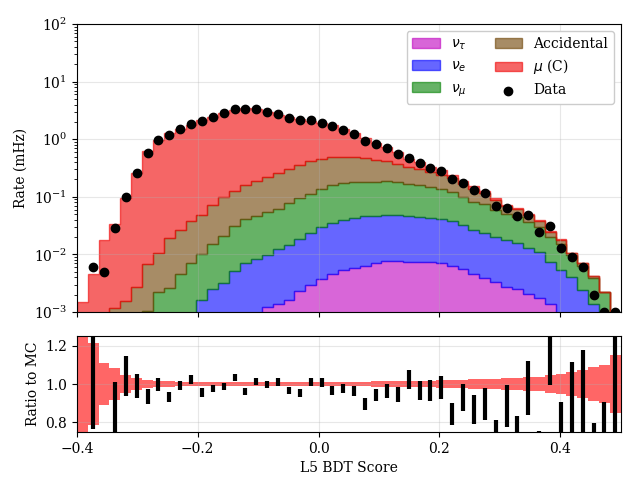
\includegraphics[width=0.9\linewidth]{BDT_Score_log.png}
		\caption[The L5 BDT Score]{The distribution of the boosted decision tree used at L5. A cut is again applied at 0.04 to remove a significant fraction of atmospheric muon background events.}
	\label{fig:L5_bdt_log}
\end{figure}

The six variables described in the GRECO Level 5 are again used to train a BDT. 
At the time of training, updated versions of both the GENIE and CORSIKA simulations were provided as part of a ongoing upgrade of the IceCube simulation.
The L5 BDT was trained using simulation files containing the then-newly available Vuvuzela V1 noise model and an updated version of the GENIE Monte Carlo generator.

A set of fifteen variables were tested.
At each step of the training, the least important variable was removed to limit the possible effects of overtraining.
The process continued until changes in the cut efficiency larger than 1\% were observed, resulting in a boost decision tree containing the six most important variables tested as described above.

The distribution of BDT score is shown in \ref{fig:L5BDT_log}. 
The data and simulation show good agreement in the muon-dominated region.
In the signal region, the data statistics is low, but the rates are consistent between data and simulation.
A cut is placed at a score of 0.04, which gives approximately 95\% background rejection with a somewhat significant hit of 30\% to all neutrino rates.

\subsection{Rates at Level 5}
\begin{table}[]
\centering
\begin{tabular}{@{}llllll@{}}
\toprule
Type         & \multicolumn{3}{l}{IceCube Processing} & GRECO  &       \\
             & Any Filter   & DC Filter  & Low-en L3  & L4     & L5    \\ \midrule
CORSIKA      & 990598       & 9178       & 969.818    & 50.511 & 4.100 \\
MuonGun      & 60669        & 2982       & 442.493    & 33.562 & 3.022 \\
Accidentals  & 35855        & 8117       & 283.559    & 11.963 & 1.799 \\
$\nu_e$      & 1.842        & 1.721      & 1.262      & 0.783  & 0.544 \\
$\nu_{\mu}$  & 11.317       & 6.360      & 4.758      & 2.503  & 1.629 \\
$\nu_{\tau}$ & 0.293        & 0.270      & 0.206      & 0.134  & 0.103 \\ \midrule
MC Total*    & 1026466      & 17303      & 1260       & 65.893 & 8.176 \\
Data         & 1154426      & 19092      & 1092       & 68.592 & 7.422 \\ \bottomrule
\end{tabular}
\caption{The event rates after the Level 5 cuts in GRECO.  The total simulated rate is calculated using CORSIKA events and ignoring MuonGun. The data rate is estimated from a burn sample of 30 runs at Level 5. Rates are given in mHz.}
\label{tab:event_rates_L5}
\end{table}

After the GRECO Level 5 cuts, the event rates for the atmospheric muons are a factor of 3x larger than the neutrino flux. 
The rate from accidental triggers in the detector is comparable to the muon neutrino rate.
The tau neutrino rate is more than an order of magnitude smaller than the muon rates, making up less than 2\% of the total rate.
Additonal cuts are needed in order to lower both sets of background below the neutrino rate.
















\graphicspath{{chapters/greco/images/level6/}}
\label{sec:level6}

\section{GRECO Level 6 Cuts}
Unlike previous levels, the GRECO L6 does not rely on a trained boosted decision tree.
The choice was made due to concerns about the significantly limited background simulation.
Such a limitation could lead to overtraining, a situation difficult to test with few simulated events.

Two cuts are applied to the sample at GRECO Level 6 for the removal of the remaining accidental triggers.
An additional three cuts are applied to reduce the muon background rate.

\subsection{Accidental Rejection at L6}

\subsubsection{Fill-Ratio at L6}
\begin{figure}[h]
	\centering
		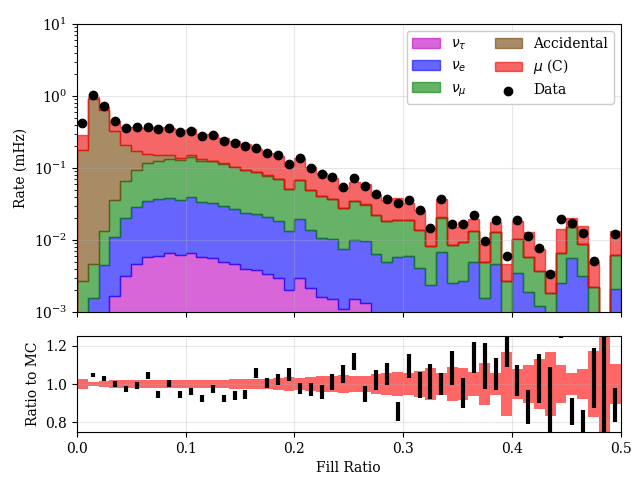
\includegraphics[width=0.9\textwidth]{FillRatio.png}
		\caption[Fill-Ratio]{The fill-ratio distribution. Note the excess of events at low values, a region dominated by the accidental triggers due to detector noise in simulation. A cut is applied at 0.05 to remove these accidental triggers.}
	\label{fig:fill-ratio}
\end{figure}

After GRECO Level 5, the accidental trigger rate is significantly larger than the expected rate of neutrinos.
While the rate of these accidental triggers is low at this stage relative to the rate at L3, they form an important background to the remaining set of neutrino events.
In order to limit their effect, two cuts are introduced to separate signal neutrinos from the accidental background.

The first of these cuts, the \emph{fill-ratio}, is a variable typically used in the search for high energy cascades \cite{IceCube-ICRC2013,IceCube-IC22-Astro} by quantifying the topology and compactness of hits within an event.

Fill-Ratio begins with a reconstructed vertex and pulse series.
In the case of the GRECO Level 6, the first hit position in DeepCore within a STW+SRT cleaned pulse series is used as an event vertex.
Both the pulse series and the event vertex are used in the fill-ratio calcuation.

A radius is computed using the provided information.
Many options are available for the caclulation of different radii, including calculations using the mean or variance of the distance between the pulses and the vertex, a parametrized radius calculation using the number of hit DOMs, and a calculation using a previously reconstructed energy.
Each configuration was tested in GRECO Level 6 with the calculation using the mean distance from the vertex showing the most promise.

\begin{equation}
	\bar{r}_{Fill-Ratio} = A \left|\frac{\sum_i^{npulses} \left(\vec{x_i}-\vec{x}_{vertex}\right)}{npulses}\right|
\end{equation}

where $A$ is a configurable scale factor. 
The algorithm next indentifies all DOMs contained with a sphere centered on the provided vertex with a radius of $\bar{r}_{Fill-Ratio}$.
The fill-ratio value is then given by the ratio of contained DOMs observing a pulse to the total number of contained DOMs.

\begin{equation}
	f = \frac{\sum_i^{ncont} \left(|\vec{r_i}\right|<\bar{r}_{Fill-Ratio} \;\&\; Q_i>0}{\sum_j^{ncont} \left(|\vec{r_j}\right|<\bar{r}_{Fill-Ratio}}
\end{equation}

This results in a measure of the compactness of a hypothetical cascade, where we expect the resulting hit distribution to be approximately spherically symmetric.
An approximately spherically symmetric cascade-like event will completely fill the fill-ratio sphere, resulting in a value near 1.0.
An extended, track-like event will have hits that are, on average, further from the starting vertex, leading to a large value of $\bar{f}_{Fill_Ratio}$, a large number of contained DOMs, and a small value of the fill-ratio.

In the context of high energy events, the fill-ratio provides good separation between cascade-like and track-like events.
Fill-ratio has not previously been used in low energy analyses, however, due to the short muon tracks of muon neutrino interactions in the 20 GeV region important for atmospheric oscillations.
At GRECO Level 6, fill-ratio has been tested to identify neutrino and atmospheric muon events with no significant separating power observed.

Sgnificant separating power was observed between the neutrino events and accidental triggers, however.
The accidental triggers include pulses throughout the detector with no clustering in the event, unlike events caused by muon or neutrino interactions, which typically have some type of clustering of pulses around the interaction position.
These events receive a large radius due to this lack of clustering and a correspondingly small value of the fill-ratio.
A choice of A=1.6 and the radius calculated using the mean distance between the first hit and all other cleaned pulses gives the separating power shown in Figure~\ref{fig:fill-ratio}.

The observed separation at a value of 0.05 allows up to one order of magnitude of reduction in the rate of accidental triggers with a relatively small reduction in signal rate of approximately 10\%.
The use of fill-ratio reduces the number of accidental triggers expected below the neutrino rate.


\subsubsection{The L6 NChannel Cut}
\begin{figure}[h]
	\centering
		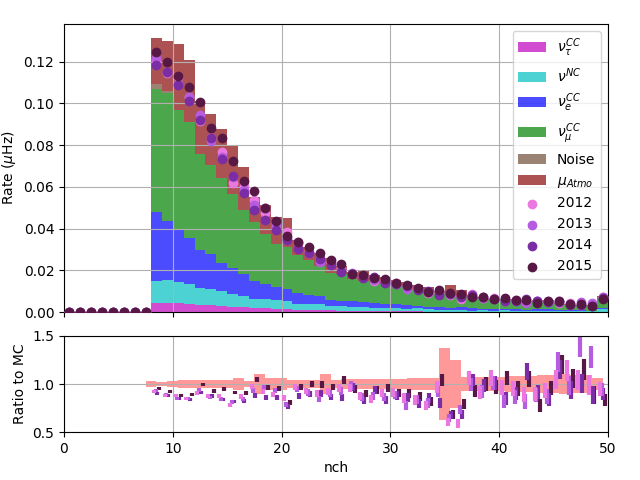
\includegraphics[width=0.9\textwidth]{nch.png}
		\caption[The NChannel Distribution]{The number of channels in the STW+SRT cleaned hit series at GRECO Level 6. At least 8 hits are required for the reconstruction performed at GRECO Level 7. Events with fewer than 8 hits are removed during Level 6, coincidentally reducing the number of accidental triggers expected.}
	\label{fig:nchannel}
\end{figure}

At GRECO Level 5, the SPE reconstruction was used to calculate the position, time, and direction of an infinite muon track.
The final reconstruction used in this analysis, Pegleg, is discussed in Section~\ref{subsec:pegleg_reco}.
Like the SPE reconstruction used at Level 5, the Pegleg reconstruction requires a minimum number of hits in order to converge.
In order to prepare for the reconstruction performed at GRECO Level 7, events with fewer than 8 hits in the STW+SRT cleaned DeepCore pulse series are removed from the selection.

This removal is performed in order to prepare for the Pegleg reconstruction, but it also removes a significant number of accidental triggers from the selection.
These events, shown in Figure~\ref{fig:nchannel}, 
The accidental triggers make up about 0.3\% of events in the sample following the combination of this cut as and the fill-ratio cut.



\subsection{Muon Rejection at L6}
\label{subsubsec:corridorcut}

\subsubsection{CorridorCut}
\begin{figure}[h]
	\centering
		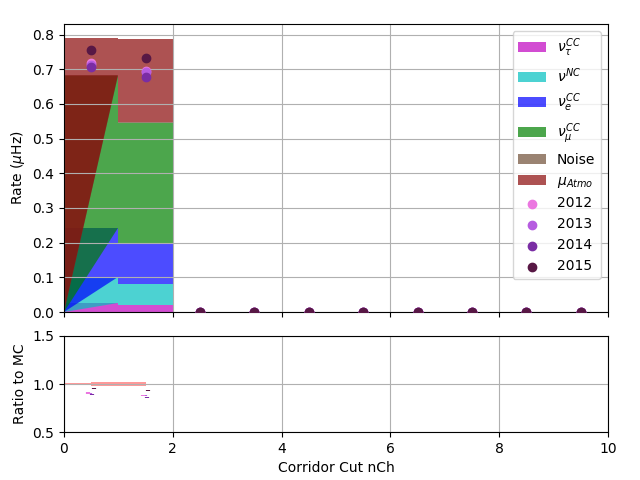
\includegraphics[width=0.9\textwidth]{Corridor_Cut_nCh.png}
		\caption[CorridorCut Distribution]{The number of channels discovered along one of the various "corridors" in the detector. Events with at least two hits discovered along a corridor are removed.}
	\label{fig:corridorcut}
\end{figure}

\begin{figure}
\centering
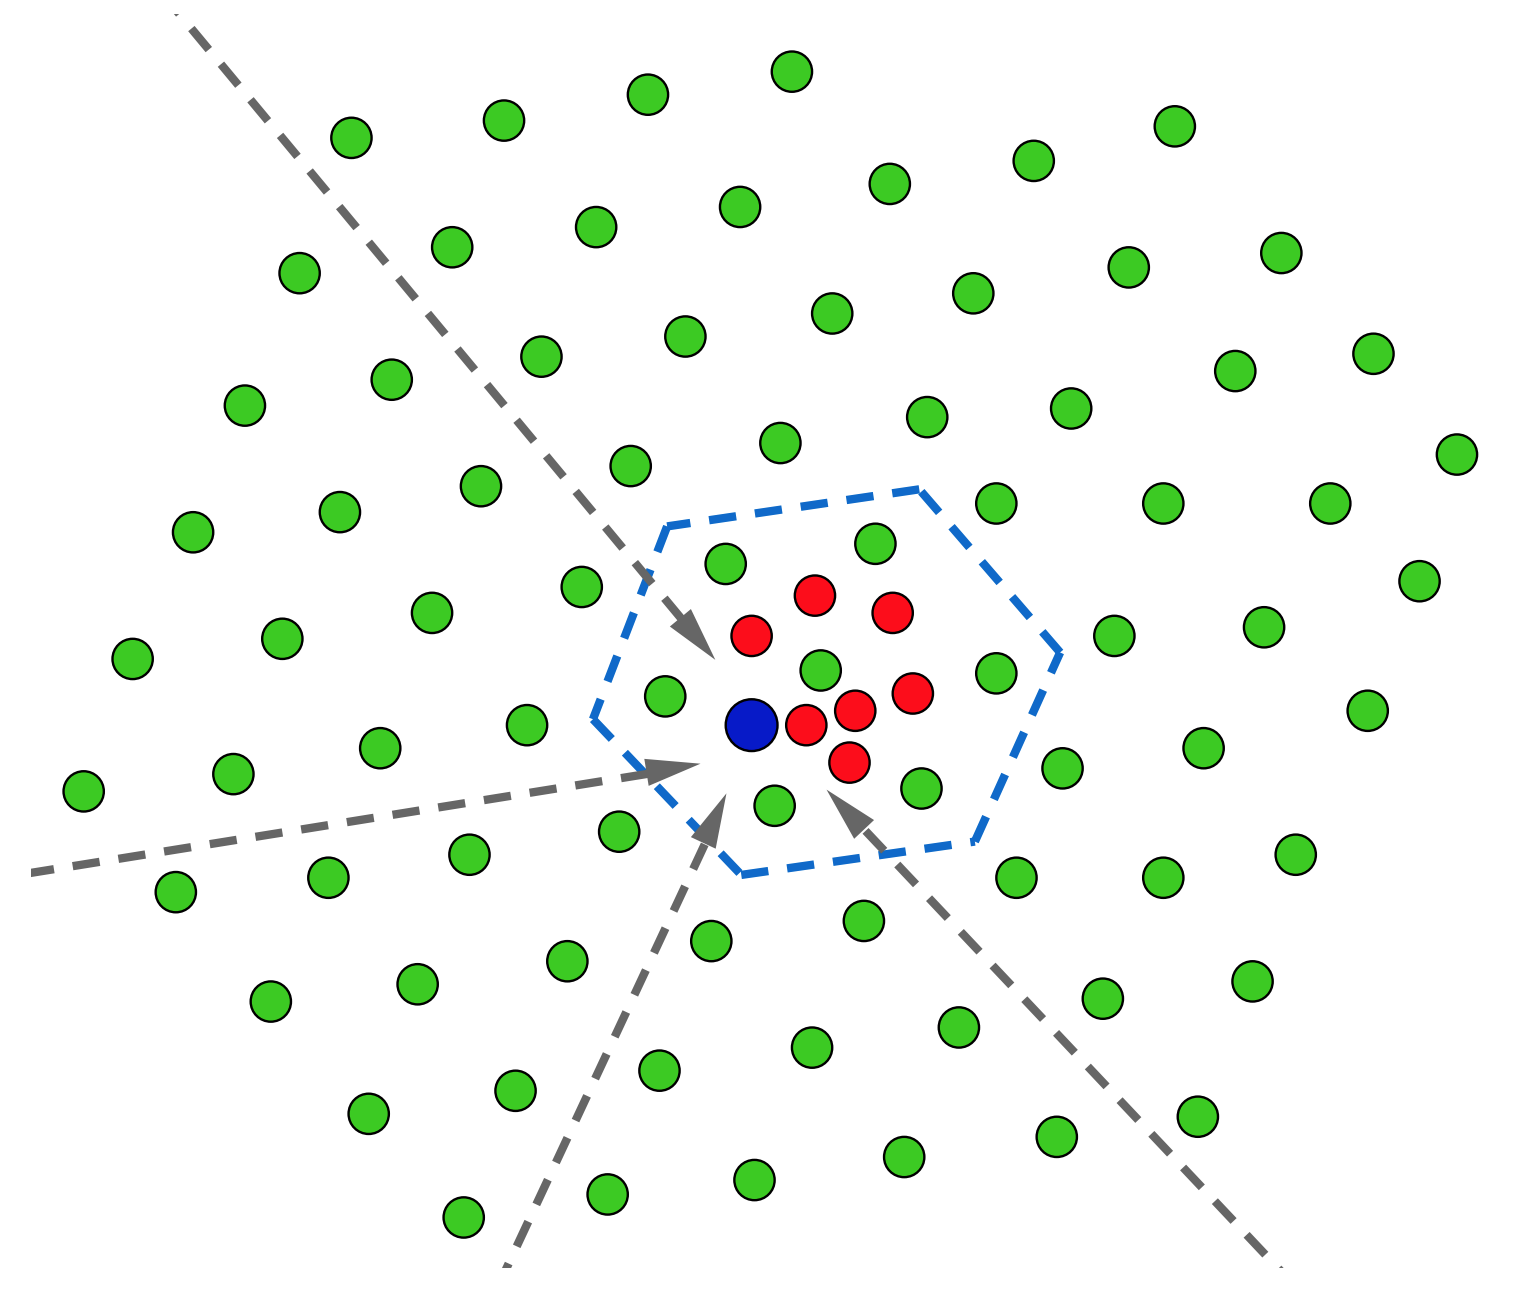
\includegraphics[width=0.7\textwidth]{corridorcut_diagram.png} 
\caption[Example of Corridors into DeepCore]{An example of "corridors" into the DeepCore fiducial volume. Muons may pass into the fiducial volume, outlined in blue, undetected by following the paths indicated by the dashed lines. Image from \cite{Thesis-Dunkman}}
\label{fig:corridorcut_diagram}
\end{figure}

The remaining atmospheric muon background after the GRECO Level 5 processing show strong selection bias, with few events remaining showing clear tracks in the veto region.
In the past, minimum-ionizing muons were discovered to be leaking into the DeepCore fiducial volume along \emph{corridors}, lines connecting the inner part of the detector to the outer edge without crossing any strings.
These events pass between strings and leave little trace in the form of identifiable hits in the outer detector.
Examples of these corridors are shown in Figure\ref{fig:corridorcut_diagram}.

In order to identify these muons, a cut was developed to look along pre-defined corridors for SLC hits correlated with pulses in DeepCore.
A CoG of the event is calculated from the STW+SRT cleaned DeepCore pulse series.
The string nearest the CoG is used to choose a set of 'corridor' strings to check for the event.
The number of hit DOMs found on the corridor strings in an uncleaned pulse series is returned.

Due to the effects of random detector noise, a cut limiting the number of discovered corridor hits to 0 would result in a significant loss of signal events.
Instead, one hit is allowed, with two or more discovered DOMs leading to the removal of the event from further processing.
At this stage, there are few events due to atmospheric muons with detectable energy in the veto, resulting in the removal of few events.
The events removed, however, are dominated by atmospheric muons, as seen in FIgure~\ref{fig:corridorcut}.

\subsubsection{FiniteReco Starting Containment}
\begin{figure}{h}%
	\centering
		\subfloat[$\rho_{FiniteReco}$]{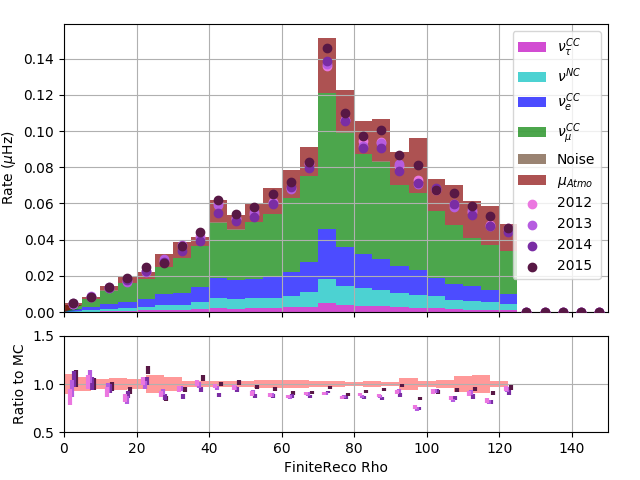
\includegraphics[width=2.3in]{FiniteReco_Rho.png}}%
		\subfloat[$Z_{FiniteReco}$]{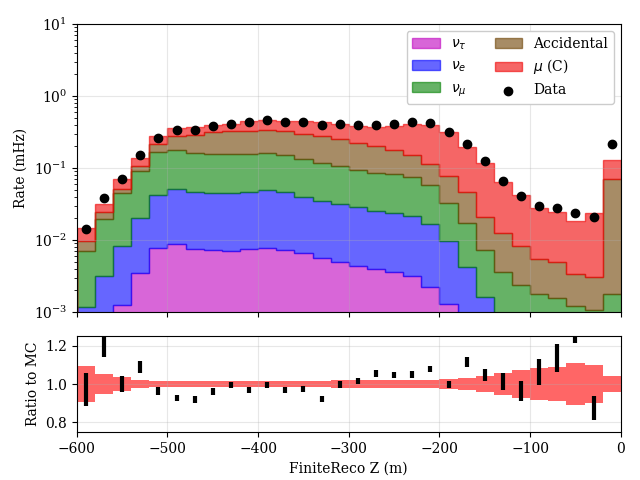
\includegraphics[width=2.3in]{FiniteReco_Z.png}}%
	\caption[The FiniteReco Containment Cuts]{The FiniteReco containment cuts. Note the exces of muons at the top and outer edge of the DeepCore fiducial volume.}%
	\label{fig:finitereco_cuts}%
\end{figure}

\begin{figure}
\centering
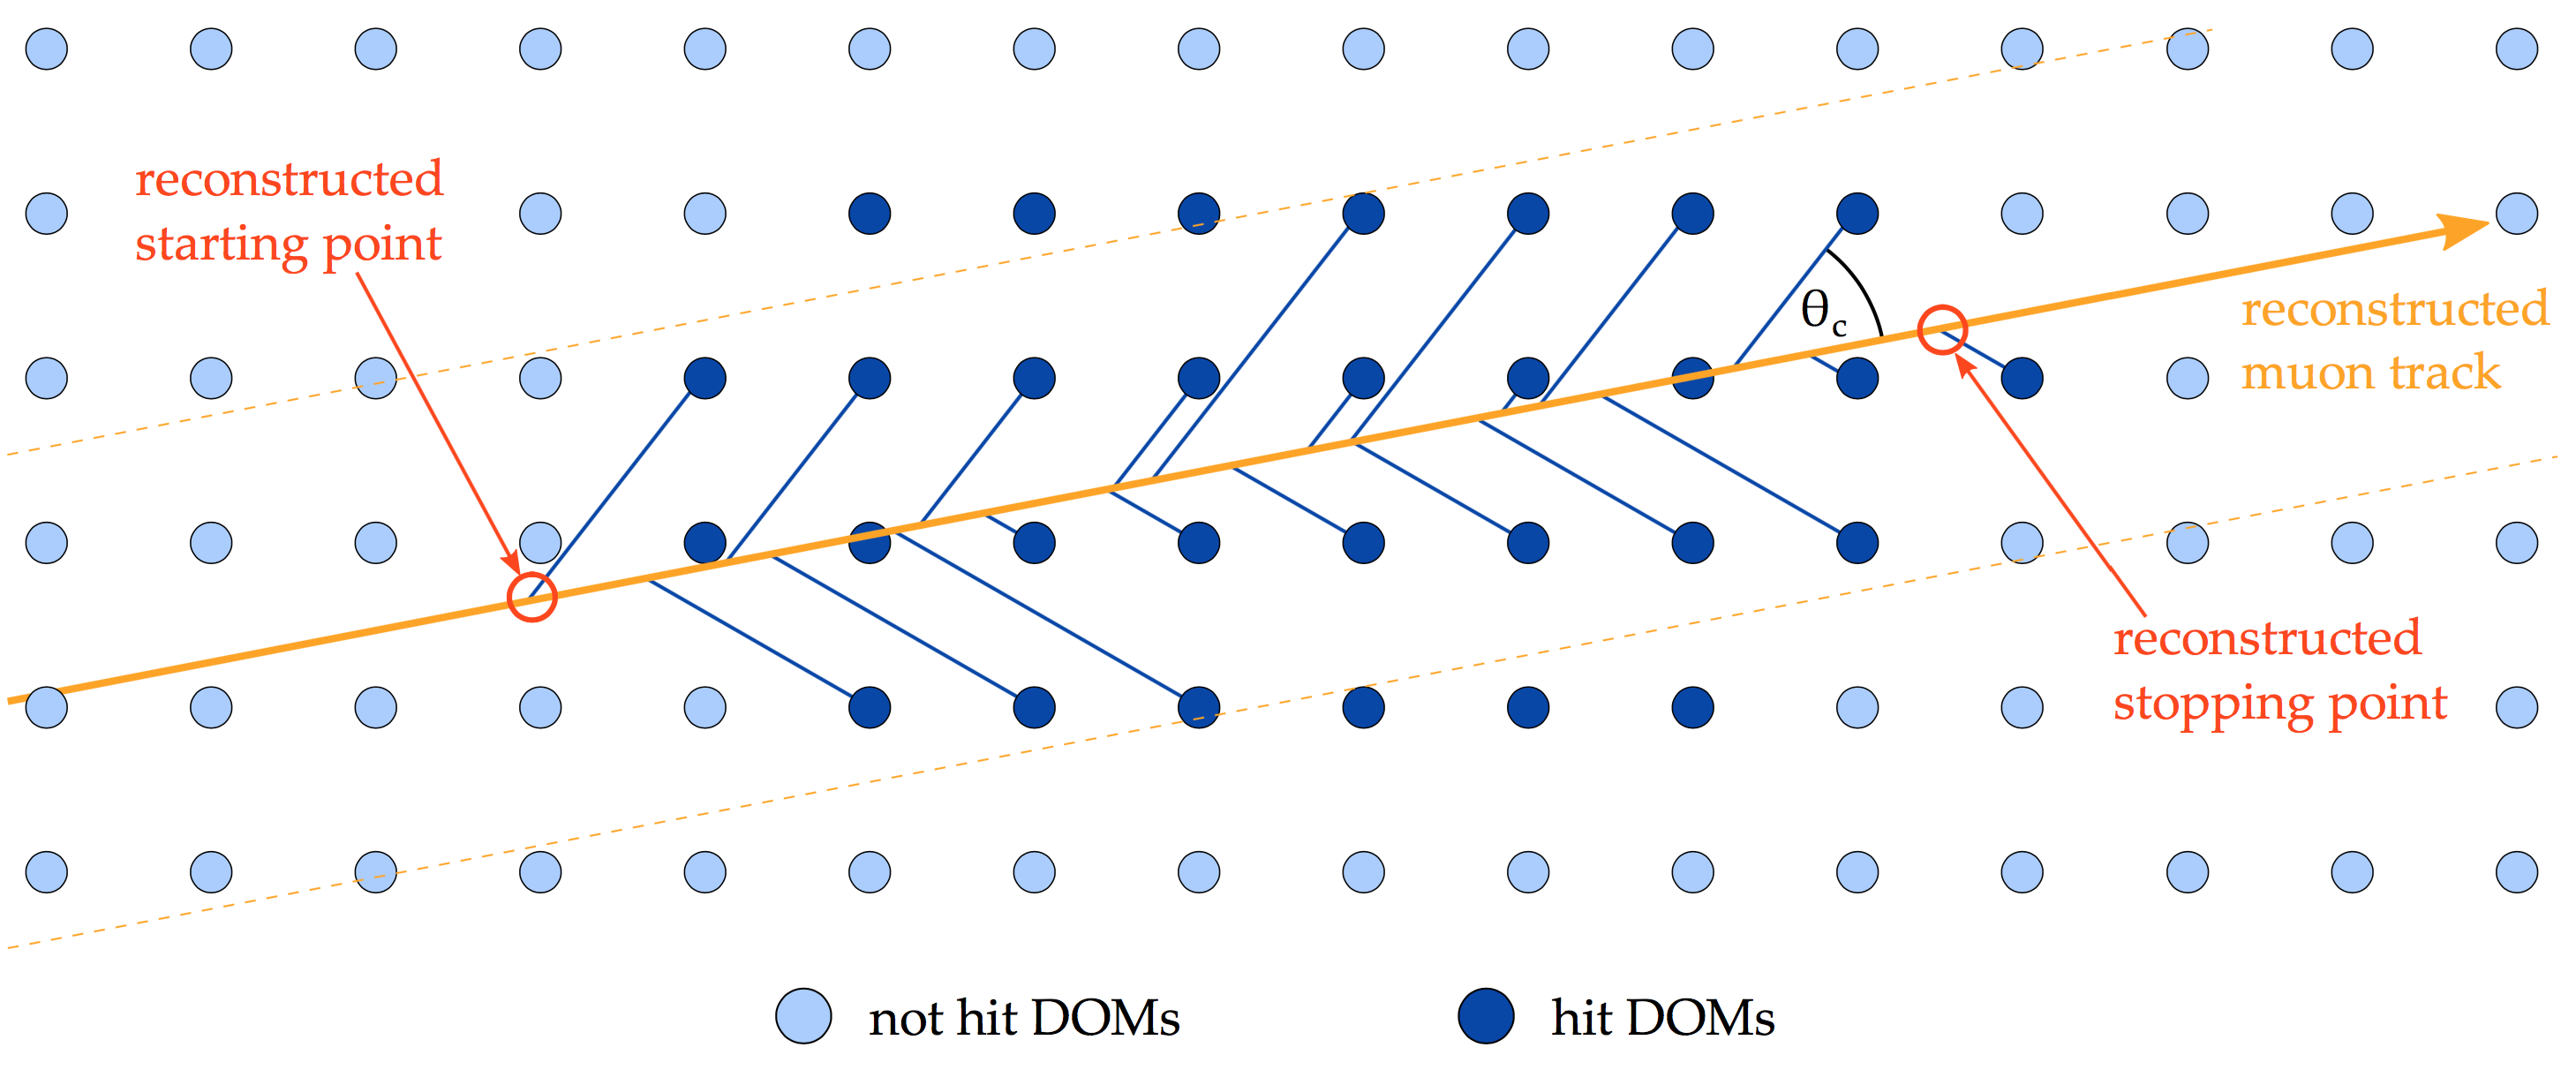
\includegraphics[width=0.9\textwidth]{finitereco_diagram.png} 
\caption[Diagram Describing the FiniteReco Method]{The FiniteReco starting and endpoint reconstruction method. FiniteReco uses an existing muon track reconstruction and the collection of hit DOMs to estimate the starting and end point of the muon track. Diagram from \cite{Thesis-Euler}.}
\label{fig:finitereco_diagram}
\end{figure}

The SPE reconstruction used in L5 was created using an infinite muon hypothesis. 
In order to refine this reconstruction, the \emph{FiniteReco} algorithm is employed.

FiniteReco is a module that accepts a previous reconstruction and a given set of pulses \cite{Thesis-Euler}.
The start and end point of the muon track may be estimated by assuming light is emitted from the track at the Cherenkov angle.
The direction of the muon track remains unchanged.
In the GRECO Level 6 processing, the SPE reconstruction from the Level 5 processing is used in the FiniteReco reconstruction.

The starting position of the resulting reconstructed particle may be used to estimate the interaction point of the particle.
Figure~\ref{fig:finitereco_zVsRho} shows the position of the reconstructed vertex in terms of depth and distance from string 36.
If an event begins outside of the DeepCore fiducial volume, the event is likely to contain a muon and can be removed from the sample.
Cuts are applied at the positions shown, resulting in a significant reduction in the number of muon events expected at final level.

\begin{center}
\begin{table}
\begin{tabular}{cc}
    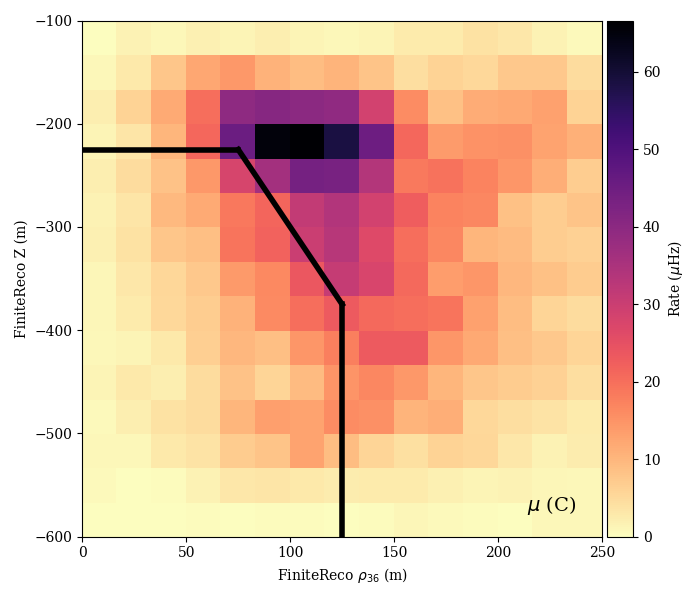
\includegraphics[width=0.45\linewidth]{z_rho_corsika.png} &  
    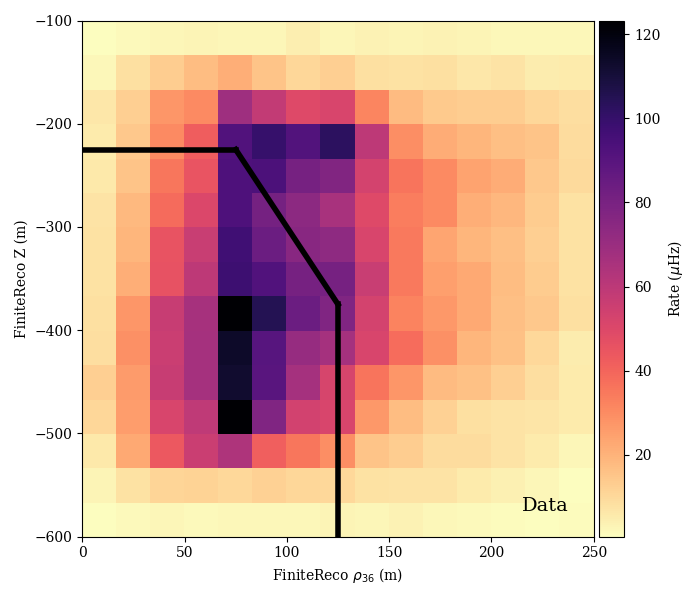
\includegraphics[width=0.45\linewidth]{z_rho_data.png} \\  

    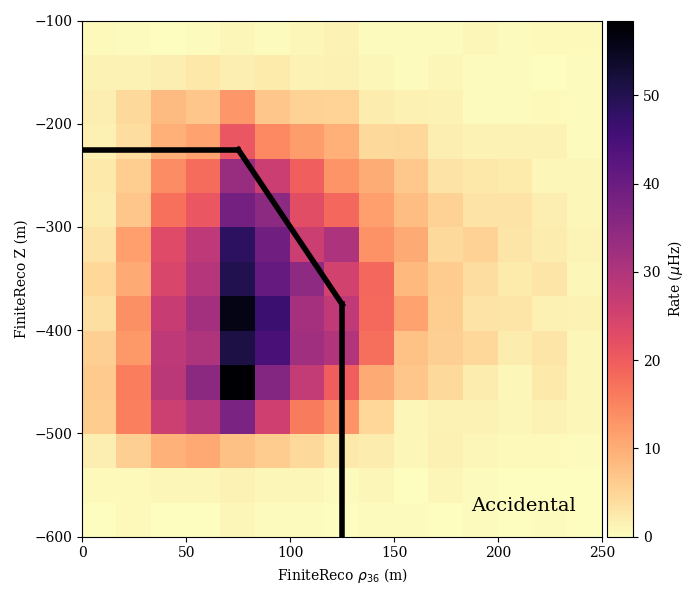
\includegraphics[width=0.45\linewidth]{z_rho_noise.png} &  
    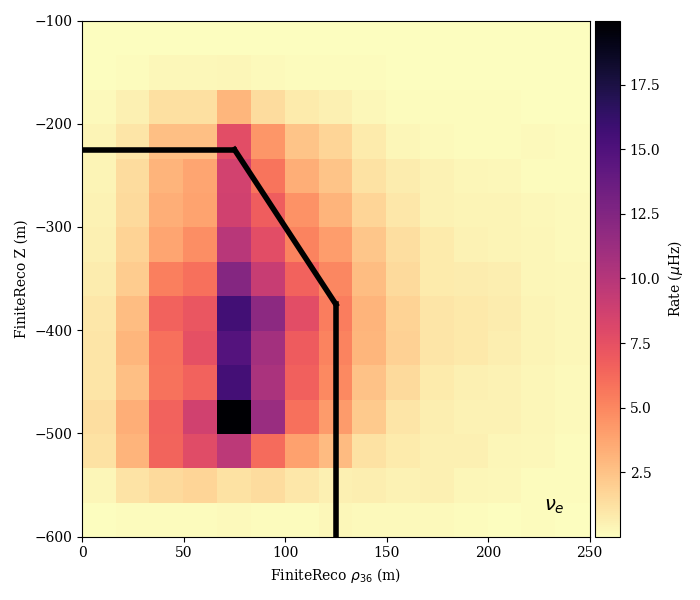
\includegraphics[width=0.45\linewidth]{z_rho_genie_nue.png} \\  

    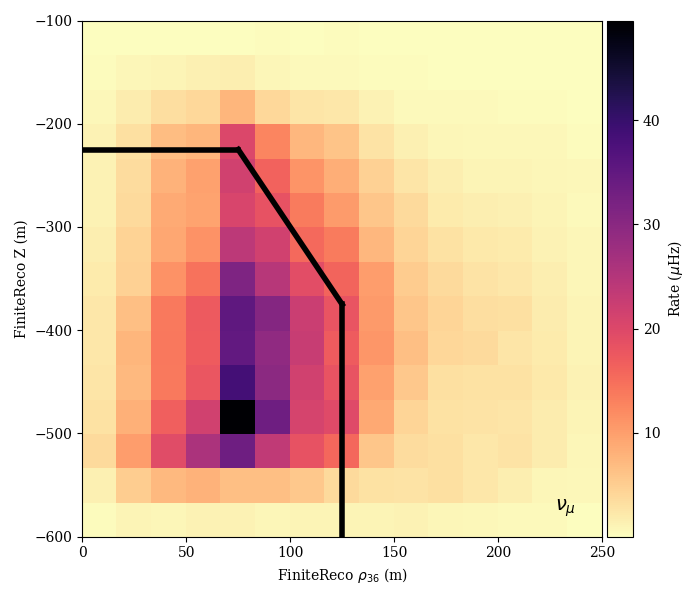
\includegraphics[width=0.45\linewidth]{z_rho_genie_numu.png} &  
    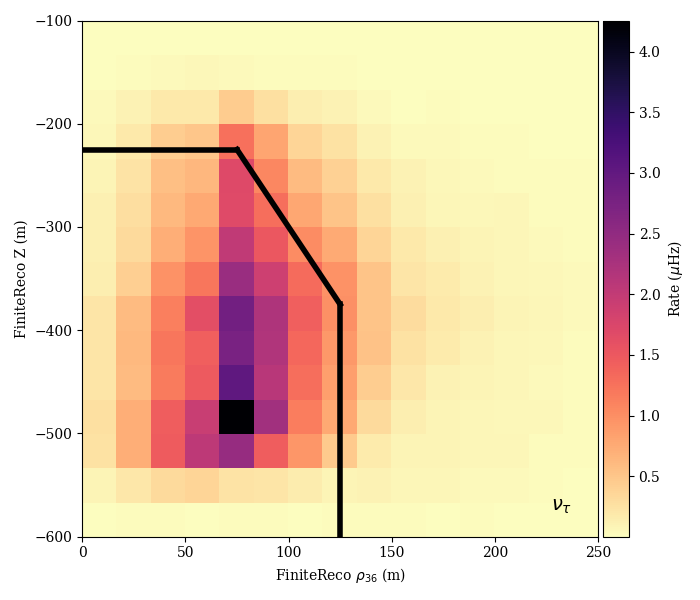
\includegraphics[width=0.45\linewidth]{z_rho_genie_nutau.png} \\ 
\end{tabular}
\label{fig:finitereco_zVsRho}
\caption[The FiniteReco containment cut applied at GRECO Level 6]{The FiniteReco containment cut for each of the channels. The cut itself is shown with the black line. The atmospheric muons, modeled with the CORSIKA generator, are reconstructed at the top of the DeepCore volume.}
\end{table}
\end{center}


\subsection{Rates at Level 6}
\begin{table}[]
\centering
\begin{tabular}{@{}lllllll@{}}
\toprule
Type         & \multicolumn{3}{l}{IceCube Processing} & \multicolumn{3}{l}{GRECO} \\
             & Any Filter   & DC Filter  & Low-en L3  & L4      & L5     & L6     \\ \midrule
CORSIKA      & 990598       & 9178       & 969.818    & 50.511  & 4.100  & 0.443  \\
MuonGun      & 60669        & 2982       & 442.493    & 33.562  & 3.022  & 0.315  \\
Accidentals  & 35855        & 8117       & 283.559    & 11.963  & 1.799  & 0.102  \\
$\nu_e$      & 1.842        & 1.721      & 1.262      & 0.783   & 0.544  & 0.362  \\
$\nu_{\mu}$  & 11.317       & 6.360      & 4.758      & 2.503   & 1.629  & 1.011  \\
$\nu_{\tau}$ & 0.293        & 0.270      & 0.206      & 0.134   & 0.103  & 0.074  \\ \midrule
MC Total*    & 1026466      & 17303      & 1260       & 65.893  & 8.176  & 1.991  \\
Data         & 1154426      & 19092      & 1092       & 68.592  & 7.422  & 1.841  \\ \bottomrule
\end{tabular}
\caption{The event rates after the Level 6 cuts in GRECO.  The total simulated rate is calculated using CORSIKA events and ignoring MuonGun. The data rate is estimated from a burn sample of 100 runs at Level 6. Rates are given in mHz.}
\label{tab:event_rates_L5}
\end{table}

After the GRECO Level 6 cuts, the sample is dominated by neutrino events.
The expected muon rate from CORSIKA simulation makes up 22\% of the total sample.
The rate from accidental events is also small, with only 5\% of events due to random detector noise.











\graphicspath{{chapters/greco/images/level7/}}
\label{sec:level7}
\graphicspath{{chapters/greco/images/level7/}}
\section{GRECO Level 7: Final Level}
The final level of the GRECO event selection, \emph{GRECO Level 7}, is the most computationally expensive stage of the selection.
While previous stages have focused on speed, using cuts based on analytic variables or on fast reconstructions using approximations to the scattering of the ice, the GRECO Level 7 employs the Pegleg reconstruction.
This reconstruction is expensive, requiring an average of 10 minutes per event.

The Pegleg reconstruction can be used to define new cuts to further reduce the atmospheric muon rates


\label{subsec:pegleg_reco}
\subsection{Reconstruction using PegLeg}
The existing reconstructions used in previous levels of the GRECO processing  use either analytic or simplified likelihood reconstructions to estimate particle parameters.
The position of the first hit and the finite muon reconstruction from FiniteReco provide separating power between atmospheric muons and neutrino events, but are designed to be computationally inexpensive instead of precise.
At final level, these estimates are refined using a novel reconstruction method developed specifically for low-energy and oscillation searches with DeepCore.

The \emph{PegLeg} reconstruction \cite{Thesis-Martin}, a refinement of previous work \cite{Thesis-Dunkman}, is a low-energy reconstruction that uses a hybrid cascade+muon hypothesis.
The reconstruction returns a total of eight parameters: the position ($x_R$, $y_R$, $z_R$), time ($t_{R}$), direction ($\theta$, $\phi$), total energy ($E_{R}$) and track length ($L_{R}$). 
The algorithm requires seeds for each of the particle parameters and a collection of hits over which to run.
Pegleg also requires a set of splines describing the expected charge as a function of distance from the emission point.
These splines are created using the CLSim module (see Section~\ref{subsec:clsim}) to direclt account for the the scattering and absorption properties of the bulk ice model.

For each particle hypothesis, the event is broken into time steps in time based on the observed pulses in the event.
At each time step, the expected charge at each DOM is calculated based on the energy and position of the particle hypothesis.
The charge expectation is evaluated for all DOMs, regardless of whether a hit is observed or not.
The total likelihood of the hypothesis is then the product of the likelihoods at each DOM.

The likelihood space itself typically possesses multiple local minima due to the small number of hits.
The fit is performed using the MultiNest minimizer package \cite{MultiNest} in order to handle the complex likelihood space.
The MultiNest algorithm calculates the likelihood for a set of 100 hypotheses at each iteration.
The likelihood at each point is used to estimate the underlying likelihood space and produces new hypotheses for testing using importance nested sampling \cite{MultiNest-ImportanceSampling}.

Given the large dimensionality of the space, significant computational power is required for the fit.
Simplifications are introduced to reduce the computational requirements of the Pegleg reconstruction.
Track lengths are limited to integer multiples of the track length used to produce the ice model spline functions.
While this requirement is lifted in newer versions of the software \cite{Thesis-Martin}, that change has not yet propagated to the current GRECO events.
In addition, only DOMs within 150 meters of the current particle position are evaluated to find the expected charge.
All other DOMs are assumed to have an expected charge consistent with noise rates.
This assumption allows the minimizer to avoid costly calculations of expected charge for distant DOMs at the expense of higher energy event resolutions.

In early versions of the PegLeg fit, the charge of individual pulses is used directly in the likelihood calculations \cite{IceCube-Millipede}.
Following the discoveries discussed in \ref{subsec:charge_templates}, however, the use of the charge was removed \cite{Thesis-Martin}}.
In the version of PegLeg used in the final version of this analysis, a deadtime window of 45 nanoseconds is introduced for each DOM directly following a pulse. 
During this window, the DOM may not contribute any further information to the fit.
This changes the reconstruction likelihood from being on the observed charge to being sensitive only to the observation or absense of charge.
Using this modification, disagreements between the data and simulated pulses resulting from mismodeling may be minimized.

Each event takes approximately 10 minutes on average to converge in the reconstruction.
There also exists a significant tail to the reconstruction time, sometimes extending to multiple hours for a single event.
With a large expected sample of events, the reconstruction time is the most computationally intensive part of the event selection. 

\label{subsec:pegleg_containment}
\subsection{Containment with PegLeg}
With a more refined reconstruction, additional constraints on the containment of the starting verticies are possible.
Similar to the work done with FiniteReco at Level 6, the reconstructed $Z$ and $\rho_{36}$ recieve cuts in two dimensions as shown in \ref{fig:pegleg_zVsRho}.
Once again, events at the top of and near the edge of DeepCore are more likely to be muons.
An additional cut is applied at the bottom of the detector in order to limit the effect of observed discrepancies between data and simulation.
Removing these events results in a 75\% reduction of the atmospheric muon background at a cost of approximately 10\% of the overall neutrino rate.

\begin{center}
\begin{table}
\begin{tabular}{cc}
    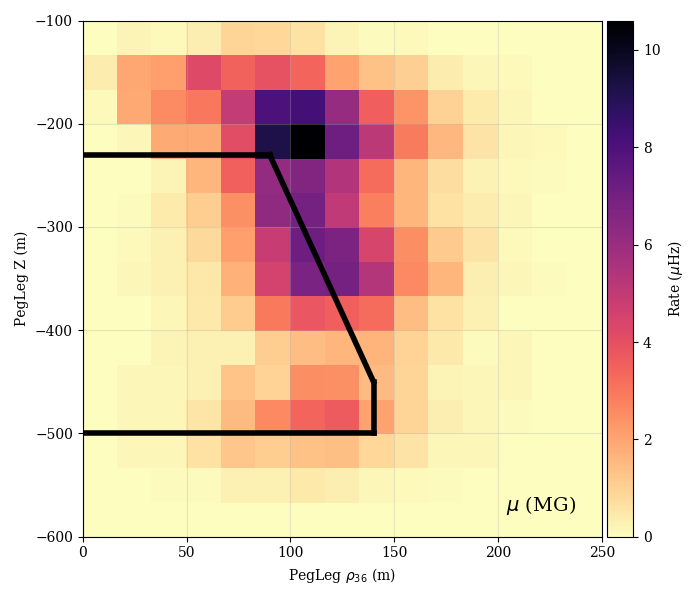
\includegraphics[width=0.45\linewidth]{pegleg_z_rho_muongun.png} &  
    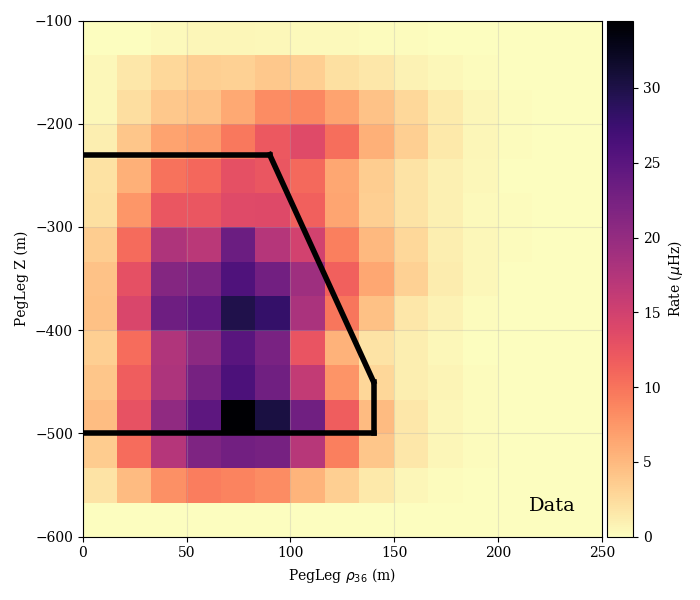
\includegraphics[width=0.45\linewidth]{pegleg_z_rho_data.png} \\  

    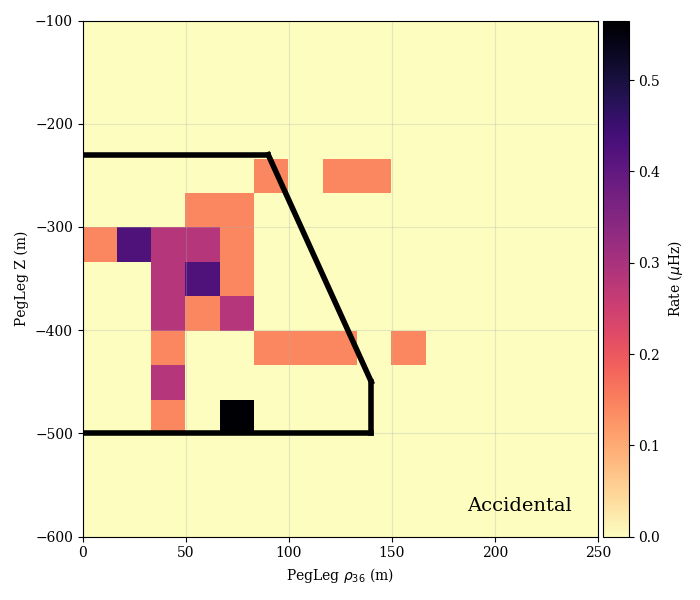
\includegraphics[width=0.45\linewidth]{pegleg_z_rho_noise.png} &  
    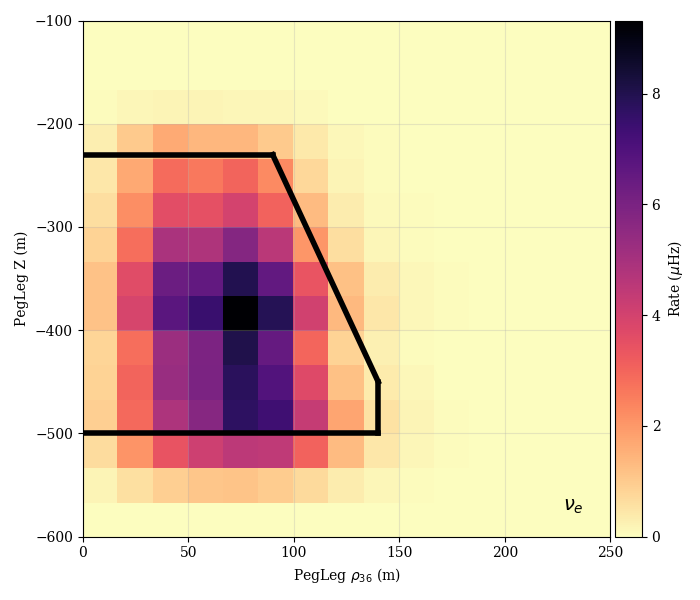
\includegraphics[width=0.45\linewidth]{pegleg_z_rho_genie_nue.png} \\  

    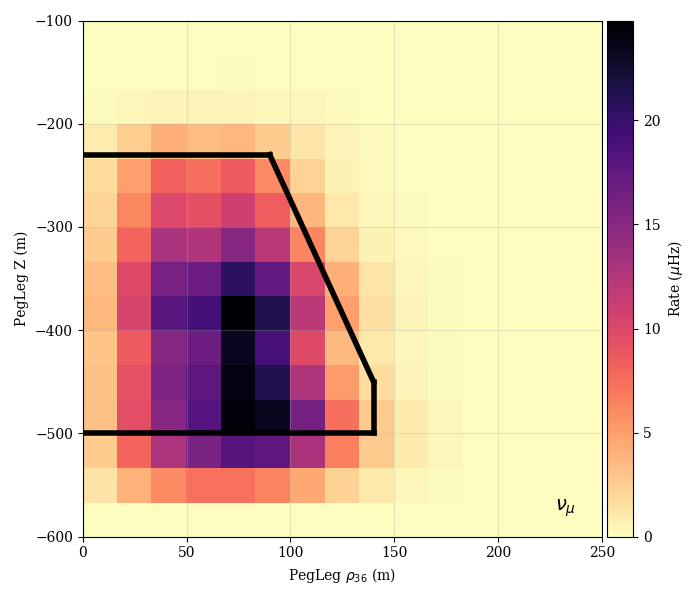
\includegraphics[width=0.45\linewidth]{pegleg_z_rho_genie_numu.png} &  
    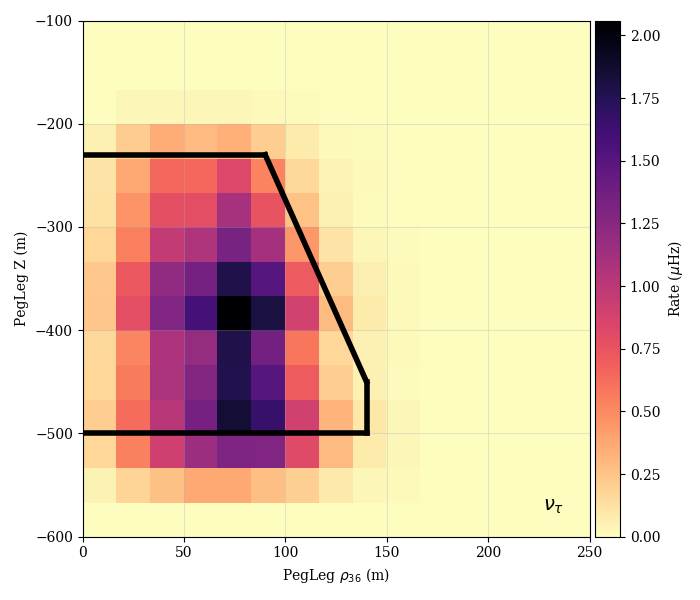
\includegraphics[width=0.45\linewidth]{pegleg_z_rho_genie_nutau.png} \\ 
\end{tabular}
\label{fig:pegleg_zVsRho}
\caption[The Pegleg containment cuts applied at Level 7]{The Pegeg L7 containment cut for each of the channels. The cut itself is shown with the black line. Note that the atmospheric muons are here represented by the higher-statistics MuonGun sample.}
\end{table}
\end{center}







\label{subsec:other_l7_cuts}
\subsection{Other Cuts at L7}
Cuts are also applied to the average reconstructed energy per hit DOM (\ref{fig:gev_per_nch}) and the scatter in the timing distribution of hits (\ref{fig:t_rms}).
The former is expected to yields high values for events dominated by flaring DOMs (Section~\ref{sec:greco_discoveries}) or events where a particle interaction occurs very close to the face of a DOM.
The distribution also shows some disagreement at low values, although good agreement between data and simulation is found for large values.

The reason for this is likely related to the issues discovered in \ref{subsubsec:charge_templates}, although this disagreement has not been investigated further.
A cut removing events with more than 3 GeV/DOM is applied only to events with fewer than 14 hits, limiting the impact on the neutrino signal events.

The scatter in the hit times shows very good agreement between data and simulation and is useful as a proxy for the overall scattering of the event.
The cut, which removes events where the standard deviation of the hit times is larger than 800 nanoseconds, is also only applied for events with fewer than 14 hits.
This limits the loss of neutrino events while removing a fraction of the remaining accidental triggers.

The cuts applied to the standard deviation in the hit times and the reconstructed energy per hit DOM are applied in two dimensions, as shown in Figure~\ref{fig:trms_ench}.


\begin{center}
\begin{table}
\begin{tabular}{cc}
    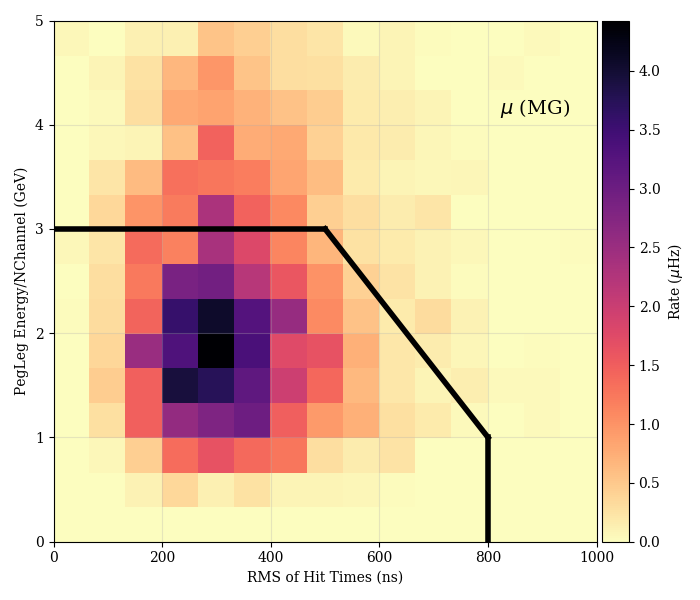
\includegraphics[width=0.45\linewidth]{pegleg_trms_ench_muongun.png} &  
    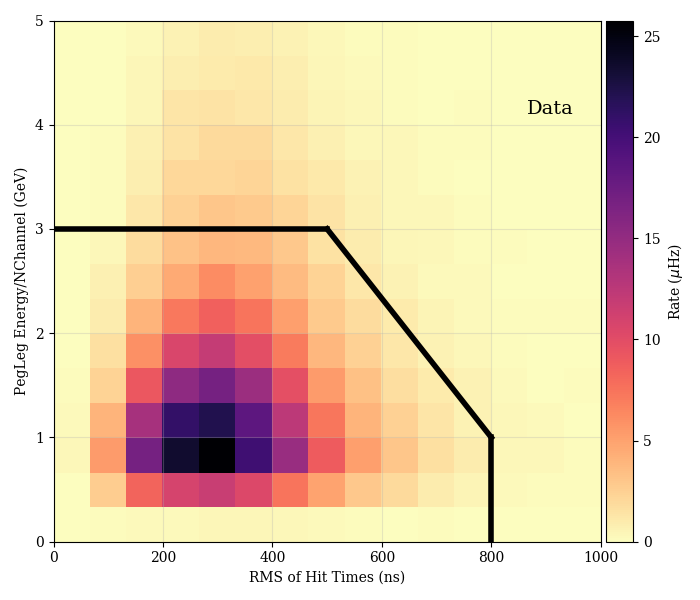
\includegraphics[width=0.45\linewidth]{pegleg_trms_ench_data.png} \\  

    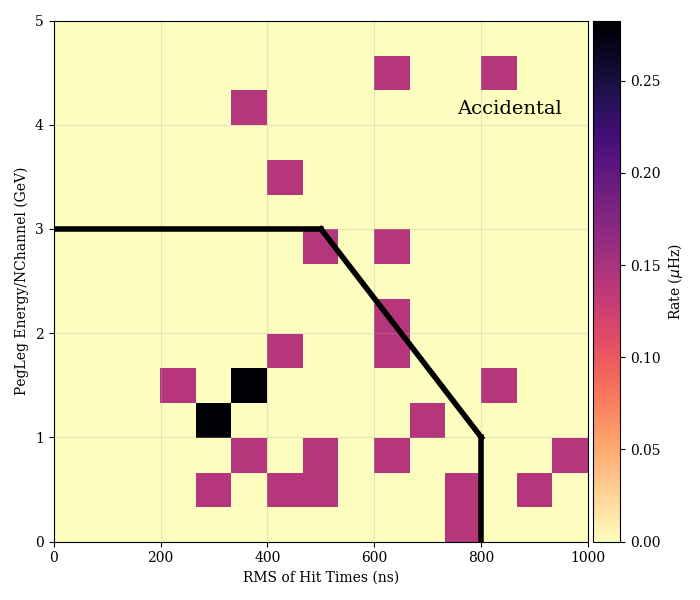
\includegraphics[width=0.45\linewidth]{pegleg_trms_ench_noise.png} &  
    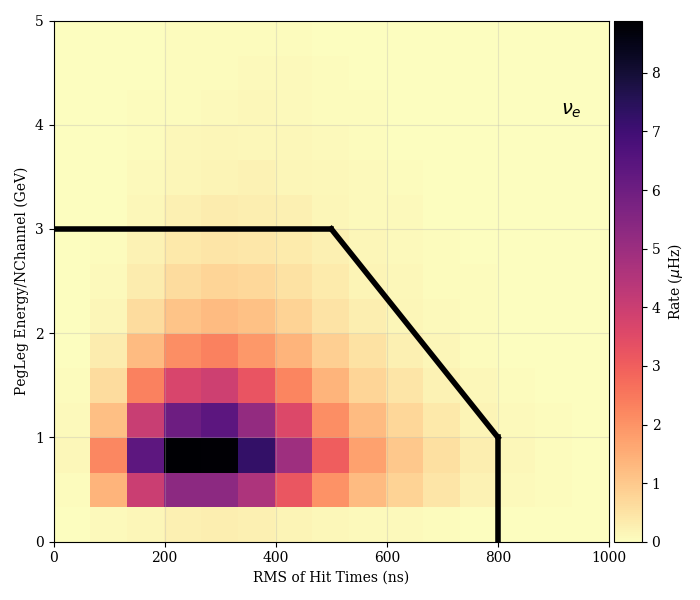
\includegraphics[width=0.45\linewidth]{pegleg_trms_ench_genie_nue.png} \\  

    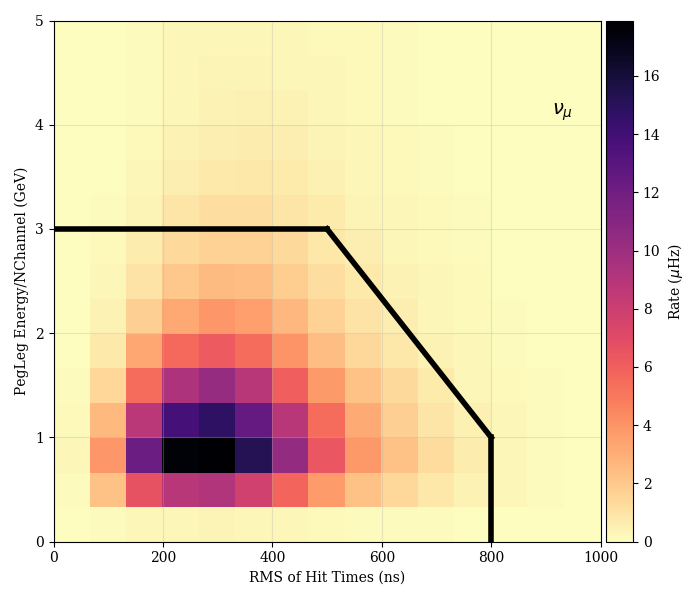
\includegraphics[width=0.45\linewidth]{pegleg_trms_ench_genie_numu.png} &  
    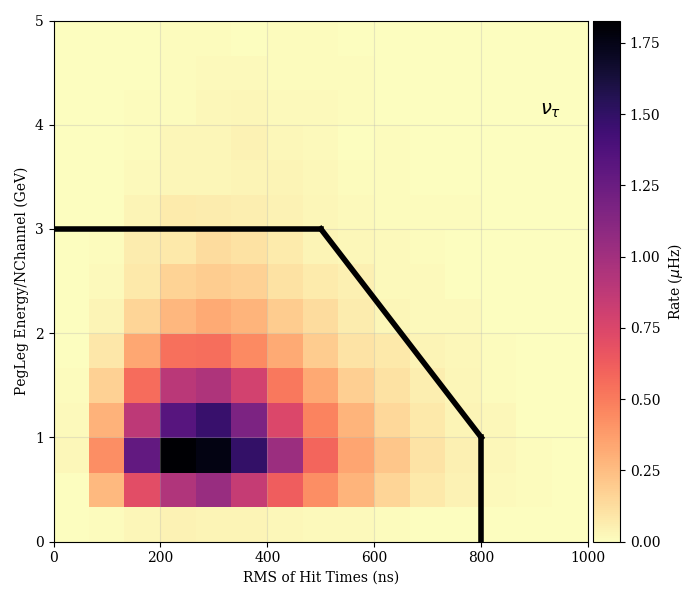
\includegraphics[width=0.45\linewidth]{pegleg_trms_ench_genie_nutau.png} \\ 
\end{tabular}
\label{fig:trms_ench}
\caption[The 2D cuts applied to the time and energy variables at Level 7]{The cuts applied to the reconstructed energy per hit DOM and the standard deviation in the hit times. The cuts are designed to remove atmospheric muons and highly scattered hits from the selection. The 2D cut shown here is applied only to hits events with fewer than 14 hit DOMs. }
\end{table}
\end{center}


















\graphicspath{{chapters/greco/images/}}
\label{sec:greco_discoveries}
\section{Calibration Discoveries with GRECO}
Checks with the GRECO analysis during the search for appearance uncovered disagreements between data and simulation.
Four sources of disagreement have been investigated further and are discussed here.
Three of these issues have not been observed in any previous selection.


\label{subsec:charge_templates}
\subsection{Disagreement in Charge Templates}

\begin{figure}
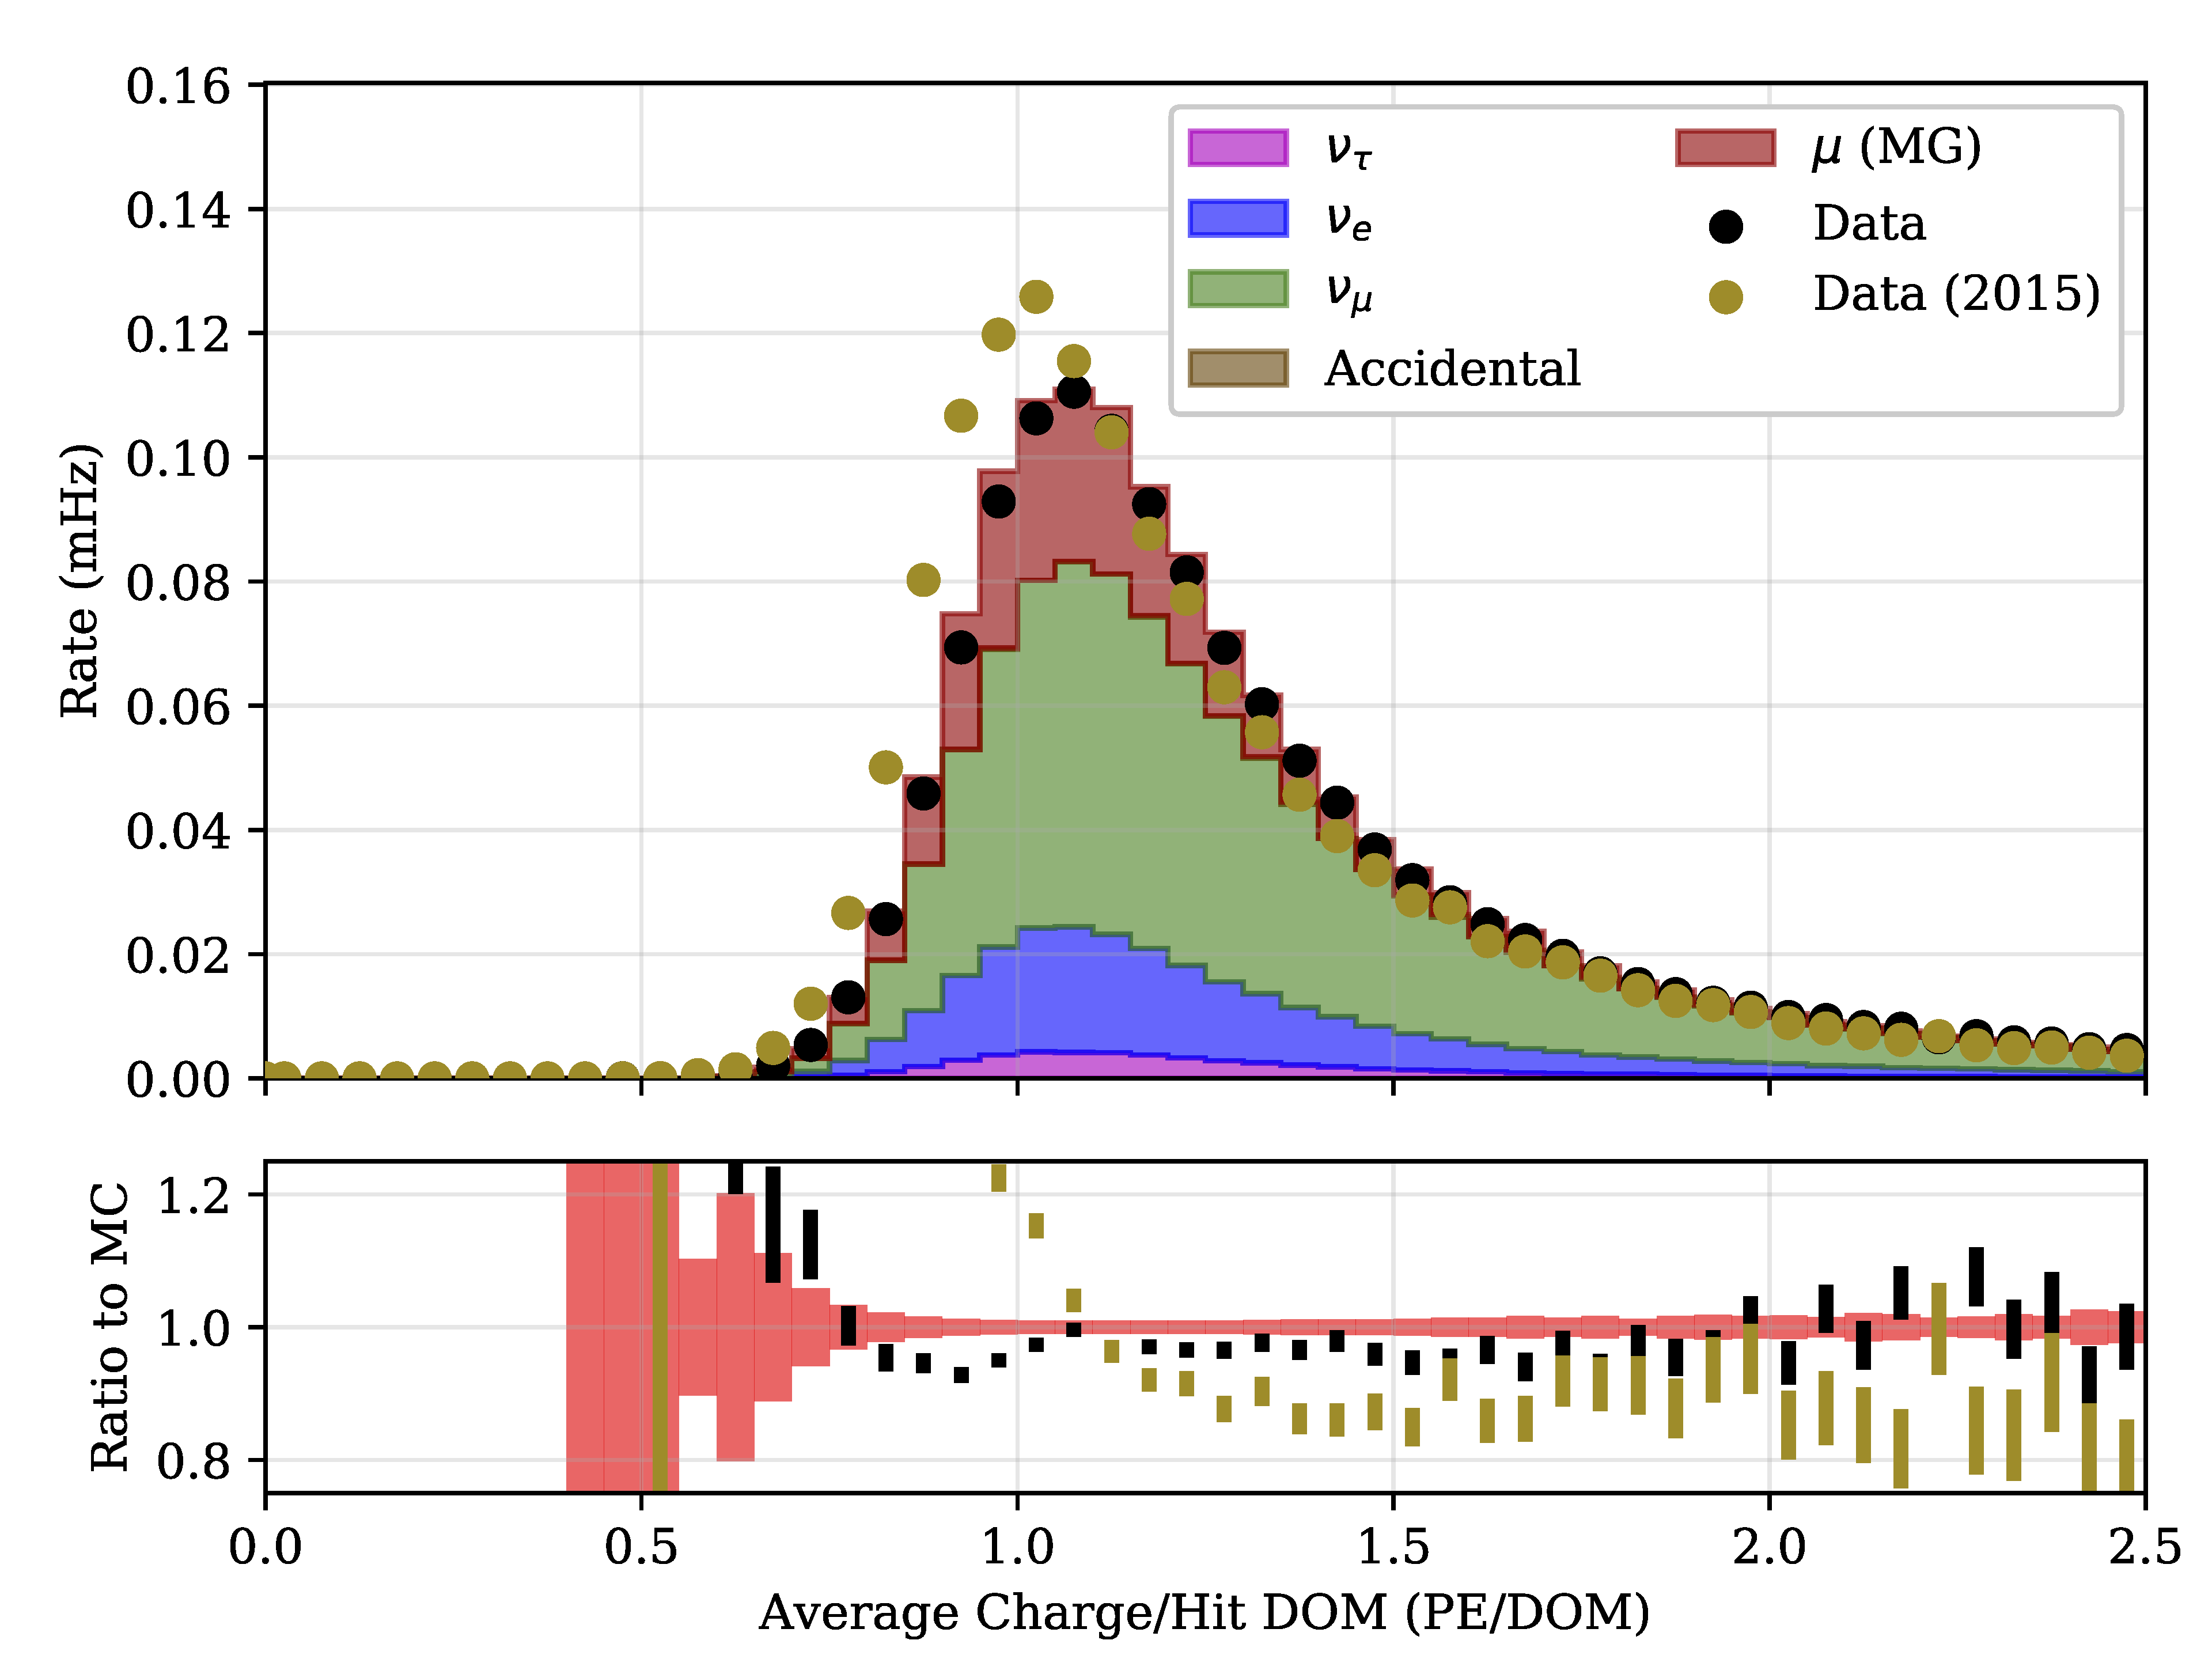
\includegraphics[width=0.9\textwidth]{L7_charge_per_channel.png} 
\end{figure}
While checking variables, significant disagreement was discovered in numerous charge variables.
A proxy for the most fundamental variable, the average charge per hit DOM, shown in \needfig{q/nch at L7}, shows systematic disagreement between the simulated events and all years of detector data.

The first suspected cause was the erroneous splitting of waveform pulses in the WaveDeform charge extraction module\findref{wavedeform?}.
The expected charge from a single incident photoelectron is used in WaveDeform to convert the digitized waveforms from the FADC and ATWD into reconstructed photoelectrons consisting of charge and timing information.
While the simulated response is known exactly, the associated charge response of the DOM in data requires careful calibration.
Using a mismodeled charge response to extract pulses in the data can result in single photoelectrons being erroneously split into multiple smaller reconstructed pulses.
Potential mismodeling effects of the charge extraction were checked in \ref{fig:pulse_timing_profile}. 
In these figures, the charge of each individual pulse is shown as a function of the arrival time, which is normalized to the time of the largest extracted pulse in the DOM for each event.

\begin{figure}
\centering
	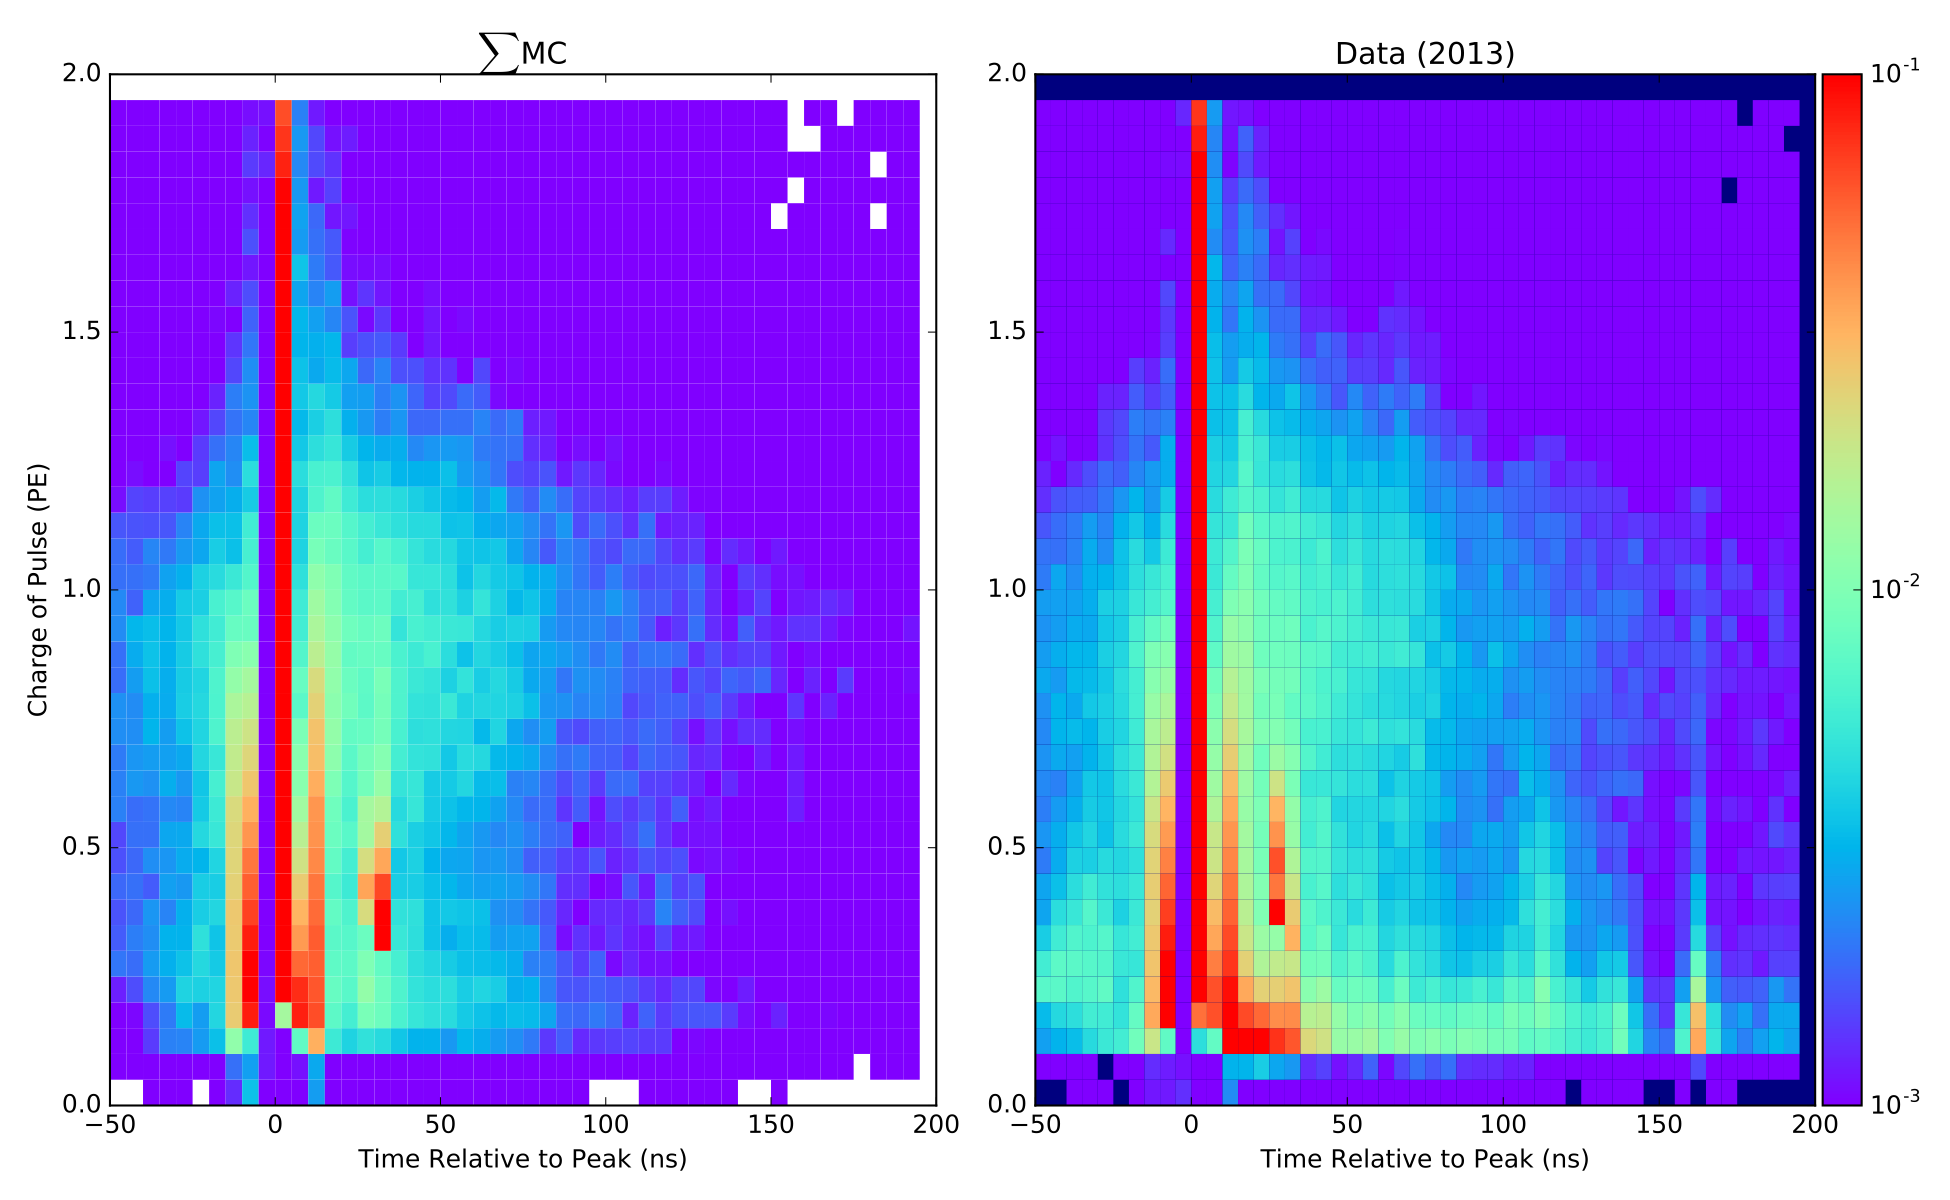
\includegraphics[width=0.9\linewidth]{2d_maps_detail_raw.png}
\label{fig:pulse_timing_profile}
\caption{A comparison of the charge extraction in data and simulation at GRECO L7. Both the time and charge are shown for individual pulses on all DOMs. The time is measured relative to the largest pulse observed on each DOM during an event. The data and simulation histograms are independently normalized to 1.0. While the two show broad agreement, notable differences occur at low charge.}
\end{figure}

Significant disagreements between the data and simulation are visible.
The erroneously split pulses are visible in data as a low-charge tail from t=0 until t=50 nanoseconds.
In addition to this effect, however, many other regions of disagreement are visible.
In data, there appear to be a significant number of prepulses not visible in the simulation occuring between t=-50 and t=-20 nanoseconds.
The structure of the late pulses, appearing with approximately 0.4 PE of charge and at time t=30 nanoseconds also appears notably different between the data and simulation.
A final set of pulses, occuring at 160 nanoseconds, also appears to be unsimulated.
This timing structure requires additional calibration resources to identify and better simulate, the scope of which is beyond this work.
Regardless, the presence of unsimulated features indicates that at least some charge information in the simulation is unreliable.

The absence of features led to investigations of the charge produced in PMTResponseSim module of DOMLauncher.
In the module, photoelectrons at the photocathode of the PMT are propagated through the dynodes to the anode.
The resulting output, a series of pulses emitted from the PMT to be passed onto the simulation of the DOM discriminator and digitization processes, requires a conversion from the number of raw incident photoelectrons to a total charge profile in the form of a waveform.
The conversion, known as the \emph{single photoelectron template}, or \emph{SPE template}, is calculated from calibration measurements performed prior to deployment of the DOMs in the ice \findref{TA003 charge template}.
The SPE template, used for all DOMs, has been known to vary somewhat between DOMs in a lab setting for many years, but the problem was deemed unimportant given other ongoing calibration work.

With the identification of the issue using the GRECO event selection, new efforts were dedicated to the production of in-situo measurements of the SPE templates for each DOM.
These new template are entering production as of the time of this analysis, but the time required for newly updated simulation is prohibitive.
Other methods are therefore necessary to avoid introducing spurious systematic biases into the final results.

In order to attempt to characterize the expected effect due to the change in the SPE templates, a new method of reweighting was developed with the GRECO selection.
The average charge per DOM, ${\bar{q}}$, is shifted by a known amount, ${\Delta \bar{q}}$ and binned.
The ratio of the shifted and unshifted average charge histograms is calculated.
An example of this process for the ${\nu_\mu^{CC}}$ is shown in \needfig{example of shifted and unshifted charges for eg numu}.
This process is performed for various values of ${\Delta \bar{q}}$ and the resulting ratios are splined using the SciPy splining function RectBivariateSpline \findref{scipy rectbivariatespline}, yielding a continuous function describing the change in the number of events at each charge as a function of ${\Delta \bar{q}}$.
This spline, an example of which is shown in \needfig{2d splines for mc charge scale correction}, may be evaluated for each event by providing the values of ${\bar{q}}$ of the given event and the ${\Delta \bar{q}}$ requested.
The output is interpreted as a rescaling factor for the event weight.

This process, referred to as \emph{MC charge rescaling}, has limitations.
In particular, threshold and selection events are completely ignored in this formulation.
A changed charge response of the detector acts roughly as a DOM efficiency shift, discussed in \ref{subsec:domeff}, which may lead to significantly different numbers of atmospheric muon background events reaching final level.
The average charge per DOM is also potentially a poor proxy if the variation in the SPE templates for each DOM is large.
Still, this process provides an estimate of the potential effect that such a correction may induce in the final event selection.
These effects are calculated and applied per-flavor, resulting in changes such as that shown in \needfig{systematic effect of mc charge scale}.

In order to verify the method, various sets of detector data were used.
Beginning with IC86-5 in the 2015-2016 operating season, the SPE templates used in the detector data were adjusted, leading to an approximately 4.5\% average shift in the expected charge.
This dataset therefore provides a known effect very similar to a recalibration of the SPE templates in Monte Carlo when compared to previous years of detector data.
The procedure described above was applied to the IC86-5 detector data and a $\chi^2$ was used to find the best-fit charge rescaling to match the IC86-2, -3, and -4 datasets.
In tests, the average expected shift between the datasets was recovered in each case, although the limitations of the method prevented a particularly strong statement about the goodness-of-fit.
This is expected due to the expected differing atmospheric muon background contributions between the earlier seasons and the IC86-5 data.
\needfig{figure 4.2.3 from my wiki}

With the verification successful, the MC charge rescaling was included as a continuous systematic in OscFit to evaluate the change in the goodness-of-fit.
Performing the blind-fit checks, the total goodness of fit was evaluted, showing a large improvement in fit quality.
The best-fit value of \unsure{find the best-fit of the mc charge scale} yielded a change in the goodness-of-fit of \unsure{what was the change in the pvalue from the mc charge scale?}.
This indicated that the MC charge rescaling could explain at least part of the disagreement observed between the data and Monte Carlo.

Due to the limitations observed in the calculation of the charge rescaling as well as the previously discussed disagreements in the simulated charge features, a decision was made to attempt to exclude the charge information from the analysis.
No changes were mandated to earlier selection levels, which showed reasonable reasonable agreement between data and Monte Carlo simulation.
Instead, this resulted in a change to the reconstruction likelihood space, excising the charge in favor of a simplified hit/not-hit model described in \ref{subsec:pegleg_reco}.
All events were reconstructed with the newly updated PegLeg reconstruction and the blind fits were reproduced.
The removal of charge information from the fit led to a significant improvement of the goodness-of-fit relative to the original blind fits on par with the introduction of the MC charge rescaling, which was made partly obsolete.

\label{subsec:flaring_doms}
\subsection{Discovery of Flaring DOMs}
Initial investigations into the poor fits in data led to comparisons of the data and Monte Carlo in various reconstructed quantities believed to be independent of the expected signal.
The decision was made to investigate these quantities using the simulation weights calculated with the baseline values.
Past experience has shown that the uncertainties in the ice model can lead to significant disagreements.
Existing uncertainties on the bulk ice assume that the coefficients for all ice layers are fully correlated.
In practice, it is possible that the ice model coefficients in parts of the detector are more poorly modeled than others.
By looking at the event rate in data and simulation as a function of the depth and position in the detector, discrepancies in the ice model can be identified.

\begin{center}
\label{fig:flaring_zrho}
\begin{figure}
	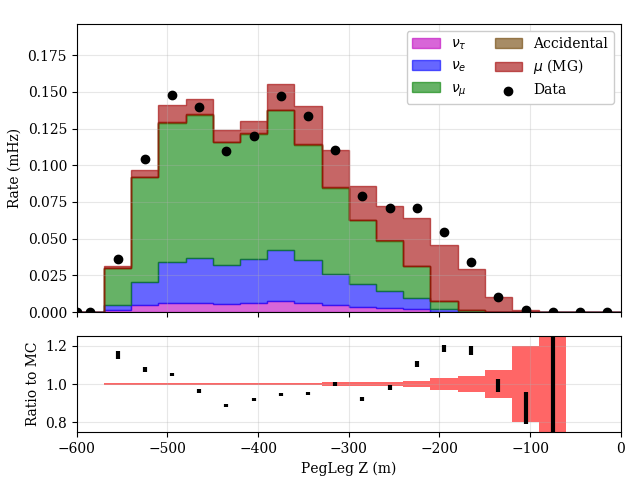
\includegraphics[width=0.6\linewidth]{L7_reco_z.png}
\caption{The reconstructed Z position using PegLeg. The GRECO L7 cuts have not been applied in order to show discrepancies below the detector. Noticeable disagreement is seen around a depth of z=-450.}
\end{figure}
\end{center}

The initial plots are shown in \ref{fig:flaring_zrho}.
A significant difference is observed at a depth of around ${Z\approx -400}$.
Checks performed with other samples have shown similar disagreeements at these depths, indicating disagreement in the ice model.
Previously unblinded oscillation samples showing this issue have not observed significant issues in the goodness-of-fit.
New ice models are underway with dedicated work to fix this region is underway.

\begin{center}
\label{fig:flaring_zrho}
\begin{figure}
	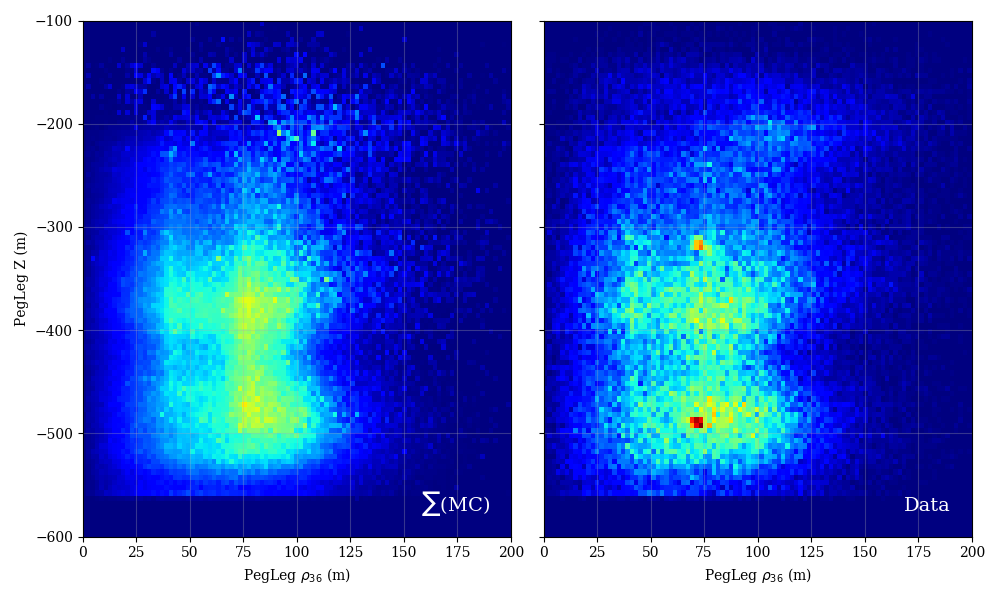
\includegraphics[width=0.9\linewidth]{pegleg_fine_z_rho.png}
\caption{The reconstructed Z position plotted against the reconstructed distance from string 36. The L7 cuts from GRECO have been removed for this plot. The colorbars in both plots have been normalized to be identical. The data and simulation show reasonable agreement except for two points in the data, near ${\rho_{36}=75}$ at depths of -310 and -490. }
\end{figure}
\end{center}

\begin{center}
\label{fig:flaring_xy}
\begin{figure}
	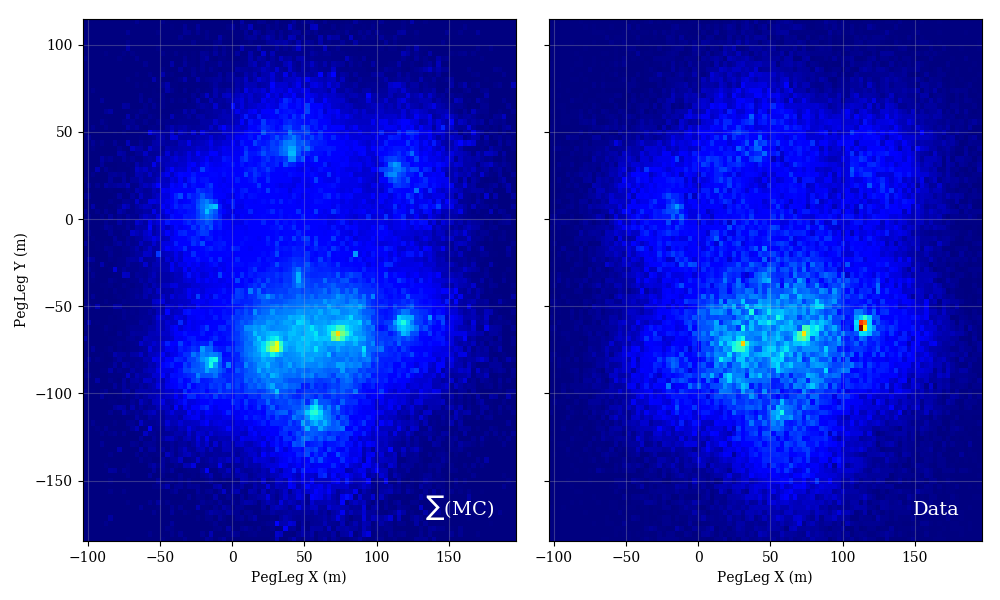
\includegraphics[width=0.9\linewidth]{pegleg_fine_x_y.png}
\caption{The reconstructed X position and Y position of events in the detector. The L7 cuts from GRECO have been removed for this plot. The colorbars in both plots have been normalized to be identical. Once again, reasonable agreement is observed in most regions, although data events have a clear excess near x=110 m, y=-60 m. This position corresponds to string 83.}
\end{figure}
\end{center}

Two-dimensional histograms of the depth and radial distance also show systematic disagreement in some regions, as shown in \ref{fig:flaring_zrho}.
These excess events appear to occur on string 83, shown in \ref{fig:flaring_xy}, indicating an effect occuring due to the DOM hardware in the detector.
Follow-up work has shown that these DOMs, known here as \emph{flaring DOMs}, appear to spontaneously emit light for unknown reasons. 
The light output is identifiable both based on the position of the hits and the amount of charge observed in nearby DOMs.
These spurious events, first discovered in the GRECO selection, have since spawned dedicated searches to better understand spontaneous light emission from the DOMs.
A small handful of DOMs have been identified by these searches with emission times as frequent as 1 Hz \findref{internal search for flaring doms}.

The affected events may be identified based on the charge profiles. 
In particular, DOMs directly adjacent to the emitting DOM observe a significant fraction of the total charge of the event.
This may be characterized using the 'charge RMS' of the event.

\label{eqn:charge_rms}
\begin{equation}
	q_{RMS} = \frac{\sigma_q}{\sum_{hits}{q_i}}
\end{equation}

\begin{center}
\begin{figure}
	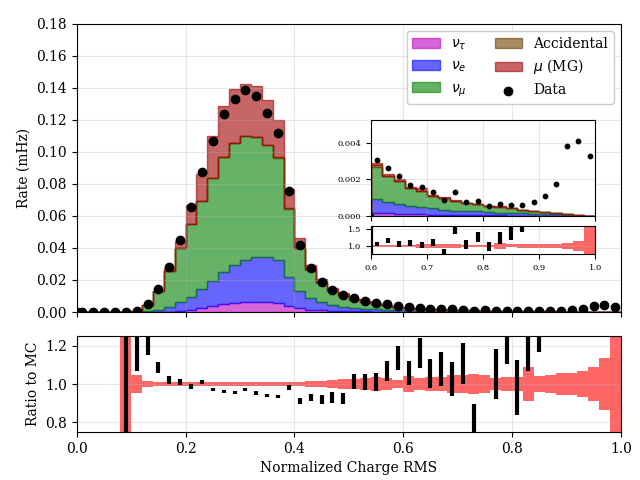
\includegraphics[width=0.9\linewidth]{L7_charge_rms_normalized.png}
\label{fig:flaring_xy}
\caption{The RMS of the charges within each event at final level. The value of the RMS is normalized using the total charge observed. The L7 cuts from GRECO are not applied here. The events with flaring DOMs cluster at high values of the charge RMS, visible in the inset.}
\end{figure}
\end{center}

This is shown in \needfig{charge rms with the excess in data}.
Events with a ${q_{RMS}}>0.85$ are removed from the analysis, removing the most obvious spurious events. 
A total of \unsure{find the number removed by the charge rms cut in data} events are removed from the GRECO data, resulting in a total reduction of \unsure{percent reduction in number of data events}\%.
The removal of these events in data and simulation does not significantly impact the goodness-of-fit of the sample due to the low event rates involved.

\label{subsec:bedrock}
\subsection{Simulation of Bedrock}
Additional disagreement was observed in the reconstructed Z position.
Near the bottom of the detector, a clear excess of events in data indicated a mismodeling in the simulation.
This disagreement increased below the detector, shown in \needfig{reco z distribution showing disagreement with data}.
Notable disagreement was also discovered in the reconstructed energy, shown in \needfig{reco energy up to a tev showing the disagreement due to bedrock}.
Events interacting below the detector may have significantly higher energies than the reconstructed energy due to the lack of instrumentation, indicating a possible connection between these two discoveries\improvement{awkward line connecting the disagreement in recoz to high reco energy}.

In the GRECO selection, events with energies above 1 TeV are modeled using NuGen simulation in order to account for events not properly simulated in the GENIE generator.
Previous investigations have shown that the two generators use similar models of the cross-section and return similar event rates at low levels.
Still, the events from the NuGen generator were shown to make up a significant fraction of the high energy tail in the GRECO sample.
These events were therefore checked for potential issues.

The NuGen and GENIE simulated event samples are used in the GRECO analyses in non-overlapping phase spaces.
The simulations do include overlapping regions, however.
For the purposes of testing, the full sample of GENIE and NuGen events were compared in true and reconstucted energy and Z position.
Initial work comparing the overlapping energy range of NuGen and GENIE events contained within the DeepCore fiducial volume showed little apparent disagreement.

Removing the constraint on the event containment, however, led to the discovery shown in \needfig{reco z of overlapping events in nugen and genie showing the bedrock problems}.
The two generators show broad agreement until a depth of approximately -830 meters, corresponding to the interface between the Antarctic glacier and the underlying bedrock.
The difference is visible in the overlapping energy range of 100 GeV to 1 TeV.

Further checks discovered the issue in IceCube's implementation of the GENIE generator.
When calculating the interaction probability for the neutrino interactions, the density of material is included.
In the implementation of GENIE previously used by the IceCube collaboration, events were assumed to occur solely within or near the fiducial volume of DeepCore due to the low energies involved.
The bedrock was therefore deemed unnecessary and not implmented in favor of assuming a uniform density of ice throughout the simulation volume.
During initial implementation, the GENIE generator was planned for use up to 100 GeV due to technical limitations. 
Later work expanded this range up to 1 TeV with future work ongoing to push toward 10 TeV.
The problems with the bedrock were mistakenly overlooked during the upgrades of the generator, leading to the systematic disagreement shown in \needfig{reference the reco z plot showing bedrock issues again}.

The bedrock has been properly included in both the NuGen generator as well as the PROPOSAL module for propagating the charged leptons.
GENIE events therefore suffer solely from an incorrect interaction probability due to the discovered bug.
The density of interaction medium enters as a linear term in the interaction probability, indicating that a correction of the form ${\rho_{rock}/\rho_{ice}}$ is sufficient to correct the Monte Carlo.
The fixed distributions in energy and zenith are shown in \needfig{energy and z distributions after reweighting genie bedrock events}.

In order to limit other potential issues from the bedrock, the analysis space was further limited, removing events both at higher energies (${E_{reco}>56 GeV}$) and those reconstructing at or below the bottom of the detector (${Z_{reco}\leq-500}$).
These cuts significantly reduce the size of the sample by reducing the high energy events included at final level. 
These changes have some impact on the expected sensitivity, but were deemed necessary to minimize the potential impact of systematics issues associated with the NuGen sample and, more broadly, limitations in the simulated event samples interacting below the detector.

\improvement{these updates with event rates should be lines on a data/mc rate table in the selection section.}

\label{sec:greco_properties}
\section{The Properties of the GRECO Event Selection}
The completion of cuts yields the completed GRECO event selection.
There are many ways to characterize the final event sample.

One of the most general methods is via the \textbf{effective area}, a theoretical construct designed to allow a generic flux to be propagated to the selection.
The effective area is a representation of the approximate cross section of a theoretical ideal detector.
By combining the effective area and an arbitrary flux, an event rate can be obtained.

The ratio of the effective area at generation level and at a later cut level gives the efficiency of the selection.
Because the event selection efficiency can change as a function of energy and direction, 

The GRECO effective area for each of the neutrino channels is shown in \ref{fig:effective_areas}.




\label{subsubsec:greco_truth}
\subsection{Energy and Zenith Reach}





Something in here about resolution, you nitwit!

\label{subsec:pegleg_containment}
\subsection{Containment with PegLeg}
